\documentclass{beamer}
%\usepackage[latin1]{inputenc}
%\usepackage{lmodern}
\usepackage{times}
\usepackage[T1]{fontenc}
\usepackage{graphicx}
\usepackage{bm}
\usepackage[small,labelformat=empty]{caption}
\usepackage{url}

\usetheme{Frankfurt}
%\usetheme{Warsaw}
\title[AllColoursAreBeautiful]{AllColoursAreBeautiful\\
{\small interactive lightinstallation inspired by blinkenlights}
}
\author[fpletz, lilafisch]{fpletz <\url{fpletz@muc.ccc.de}>,\\ lilafisch <\url{lilafisch@muc.ccc.de}>}
\institute[$\mu c^{3}$]{$\mu c^{3}$ - CCC Munich }
\date{2010-12-27 - Day 1 @ 27C3}

\begin{document}

{
%\usebackgroundtemplate{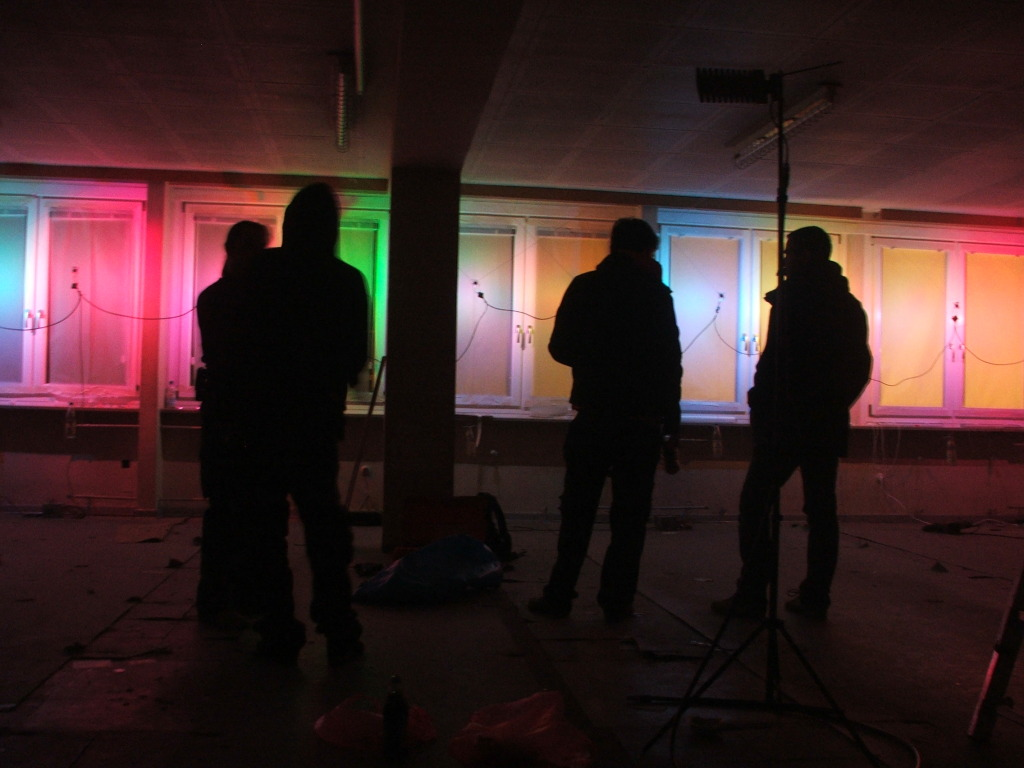
\includegraphics[width=\paperwidth]{bilder/behindthescreen.jpg}}
\begin{frame}
\thispagestyle{empty}
\titlepage
\end{frame}
}

\begin{frame}
\frametitle{Fahrplan}
\tableofcontents
\end{frame}

\setlength\fboxsep{5pt}
\setlength\fboxrule{0pt}

\section{$\mu c^{3}$}
  \begin{frame}{$\mu c^{3}$}
    \begin{columns}%[t]
      \begin{column}{5cm}
        \begin{block}{info}
         Chaos Computer Club M\"unchen
               \begin{itemize}
            \item e.V. founded in 1999
            \item > 80 members
                  \item http://muc.ccc.de
                  \item info@muc.ccc.de
            \end{itemize}
        \end{block}
%         \begin{figure}
%          \begin{center}
%          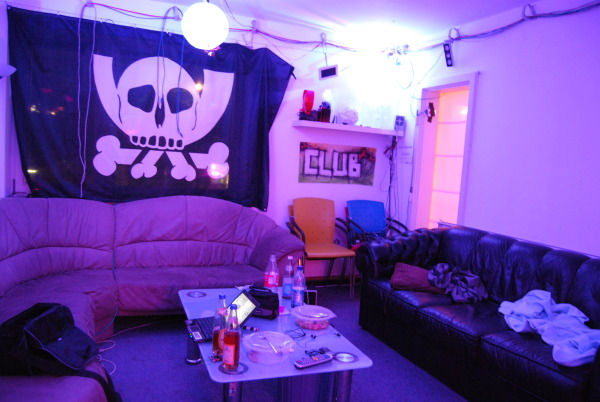
\includegraphics[width=5cm]{bilder/hbf.jpg}
%          \end{center}
%        \end{figure}

%         \begin{figure}
 %           \begin{center}
 %           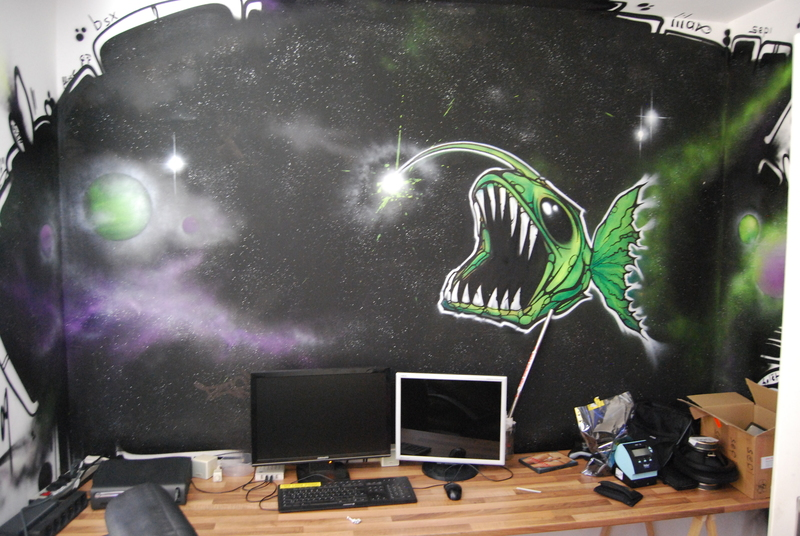
\includegraphics[width=2cm]{bilder/maxi.jpg}
 %           \end{center}
 %         \end{figure}
      \end{column}
      \begin{column}{5cm}
        \begin{figure}
          \begin{center}
          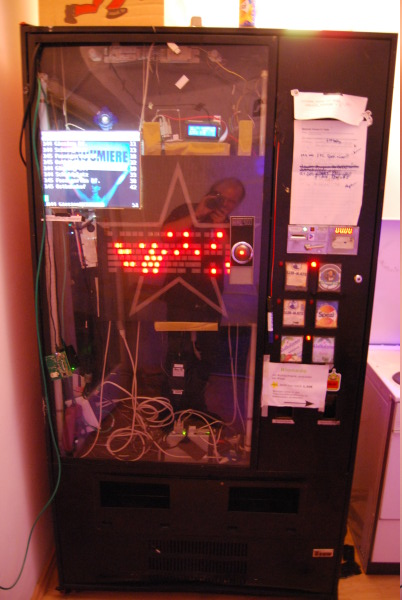
\includegraphics[width=4cm]{bilder/matemat.jpg}
%         \caption{\small matemat}
          \end{center}
        \end{figure}
%        \begin{figure}
%          \begin{center}
%          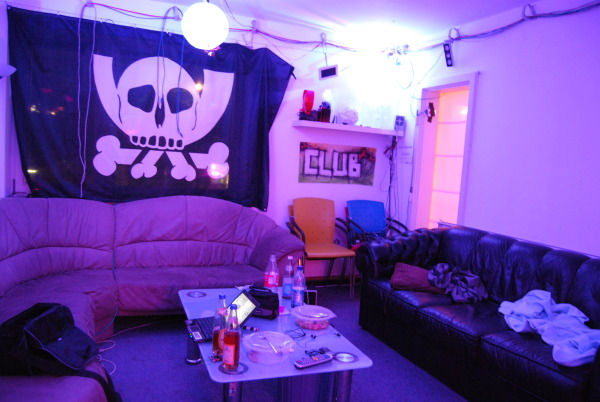
\includegraphics[width=3cm]{bilder/hbf.jpg}
%          \end{center}
%        \end{figure}
      \end{column}
    \end{columns}
    \end{frame}
\section{History}
\begin{frame}{How it came together}

\begin{columns}%[T]
\begin{column}{3.5cm}
        \begin{figure}
          \begin{center}
          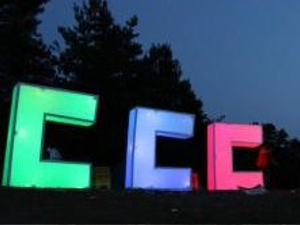
\includegraphics[width=3cm]{bilder/ddc_har.jpg}
          \caption{Moodlamp}
         % members' RGB-LED project, \\were in use for the 3c
          \end{center}
        \end{figure}
\end{column}
\begin{column}{3.5cm}
        \begin{figure}
          \begin{center}
          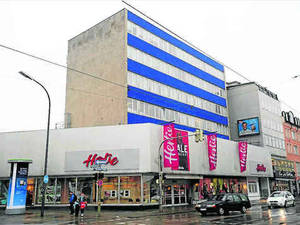
\includegraphics[width=3cm]{bilder/hertie.jpg}
          \caption{Puerto Giesing}
          %old office building,\\used by artists before beeing torn down
          \end{center}
        \end{figure}
\end{column}
\begin{column}{3.5cm}
        \begin{figure}
          \begin{center}
          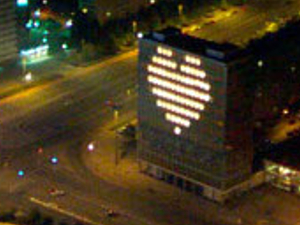
\includegraphics[width=3cm]{bilder/blinkenlights.jpg}
          \caption{Blinkenlights}
          %well known project transforming buildings into b/w displays
          \end{center}
        \end{figure}
\end{column}
\end{columns}
\begin{columns}[T]
\begin{column}{3.5cm}
        \begin{figure}
          \begin{center}
          $\mu c^3$'s RGB-LED project, i.e. in use for the 3c
          \end{center}
        \end{figure}

\end{column}
\begin{column}{3.5cm}
        \begin{figure}
          \begin{center}
          Old office building,\\used by artists before beeing torn down
          \end{center}
        \end{figure}

\end{column}
\begin{column}{3.5cm}
        \begin{figure}
          \begin{center}
          Well known project transforming buildings into b\textbackslash w displays
          \end{center}
        \end{figure}

    \end{column}
\end{columns}
\end{frame}

\begin{frame}{Unexpected Challenges}
  \begin{columns}
    \begin{column}{6cm}
        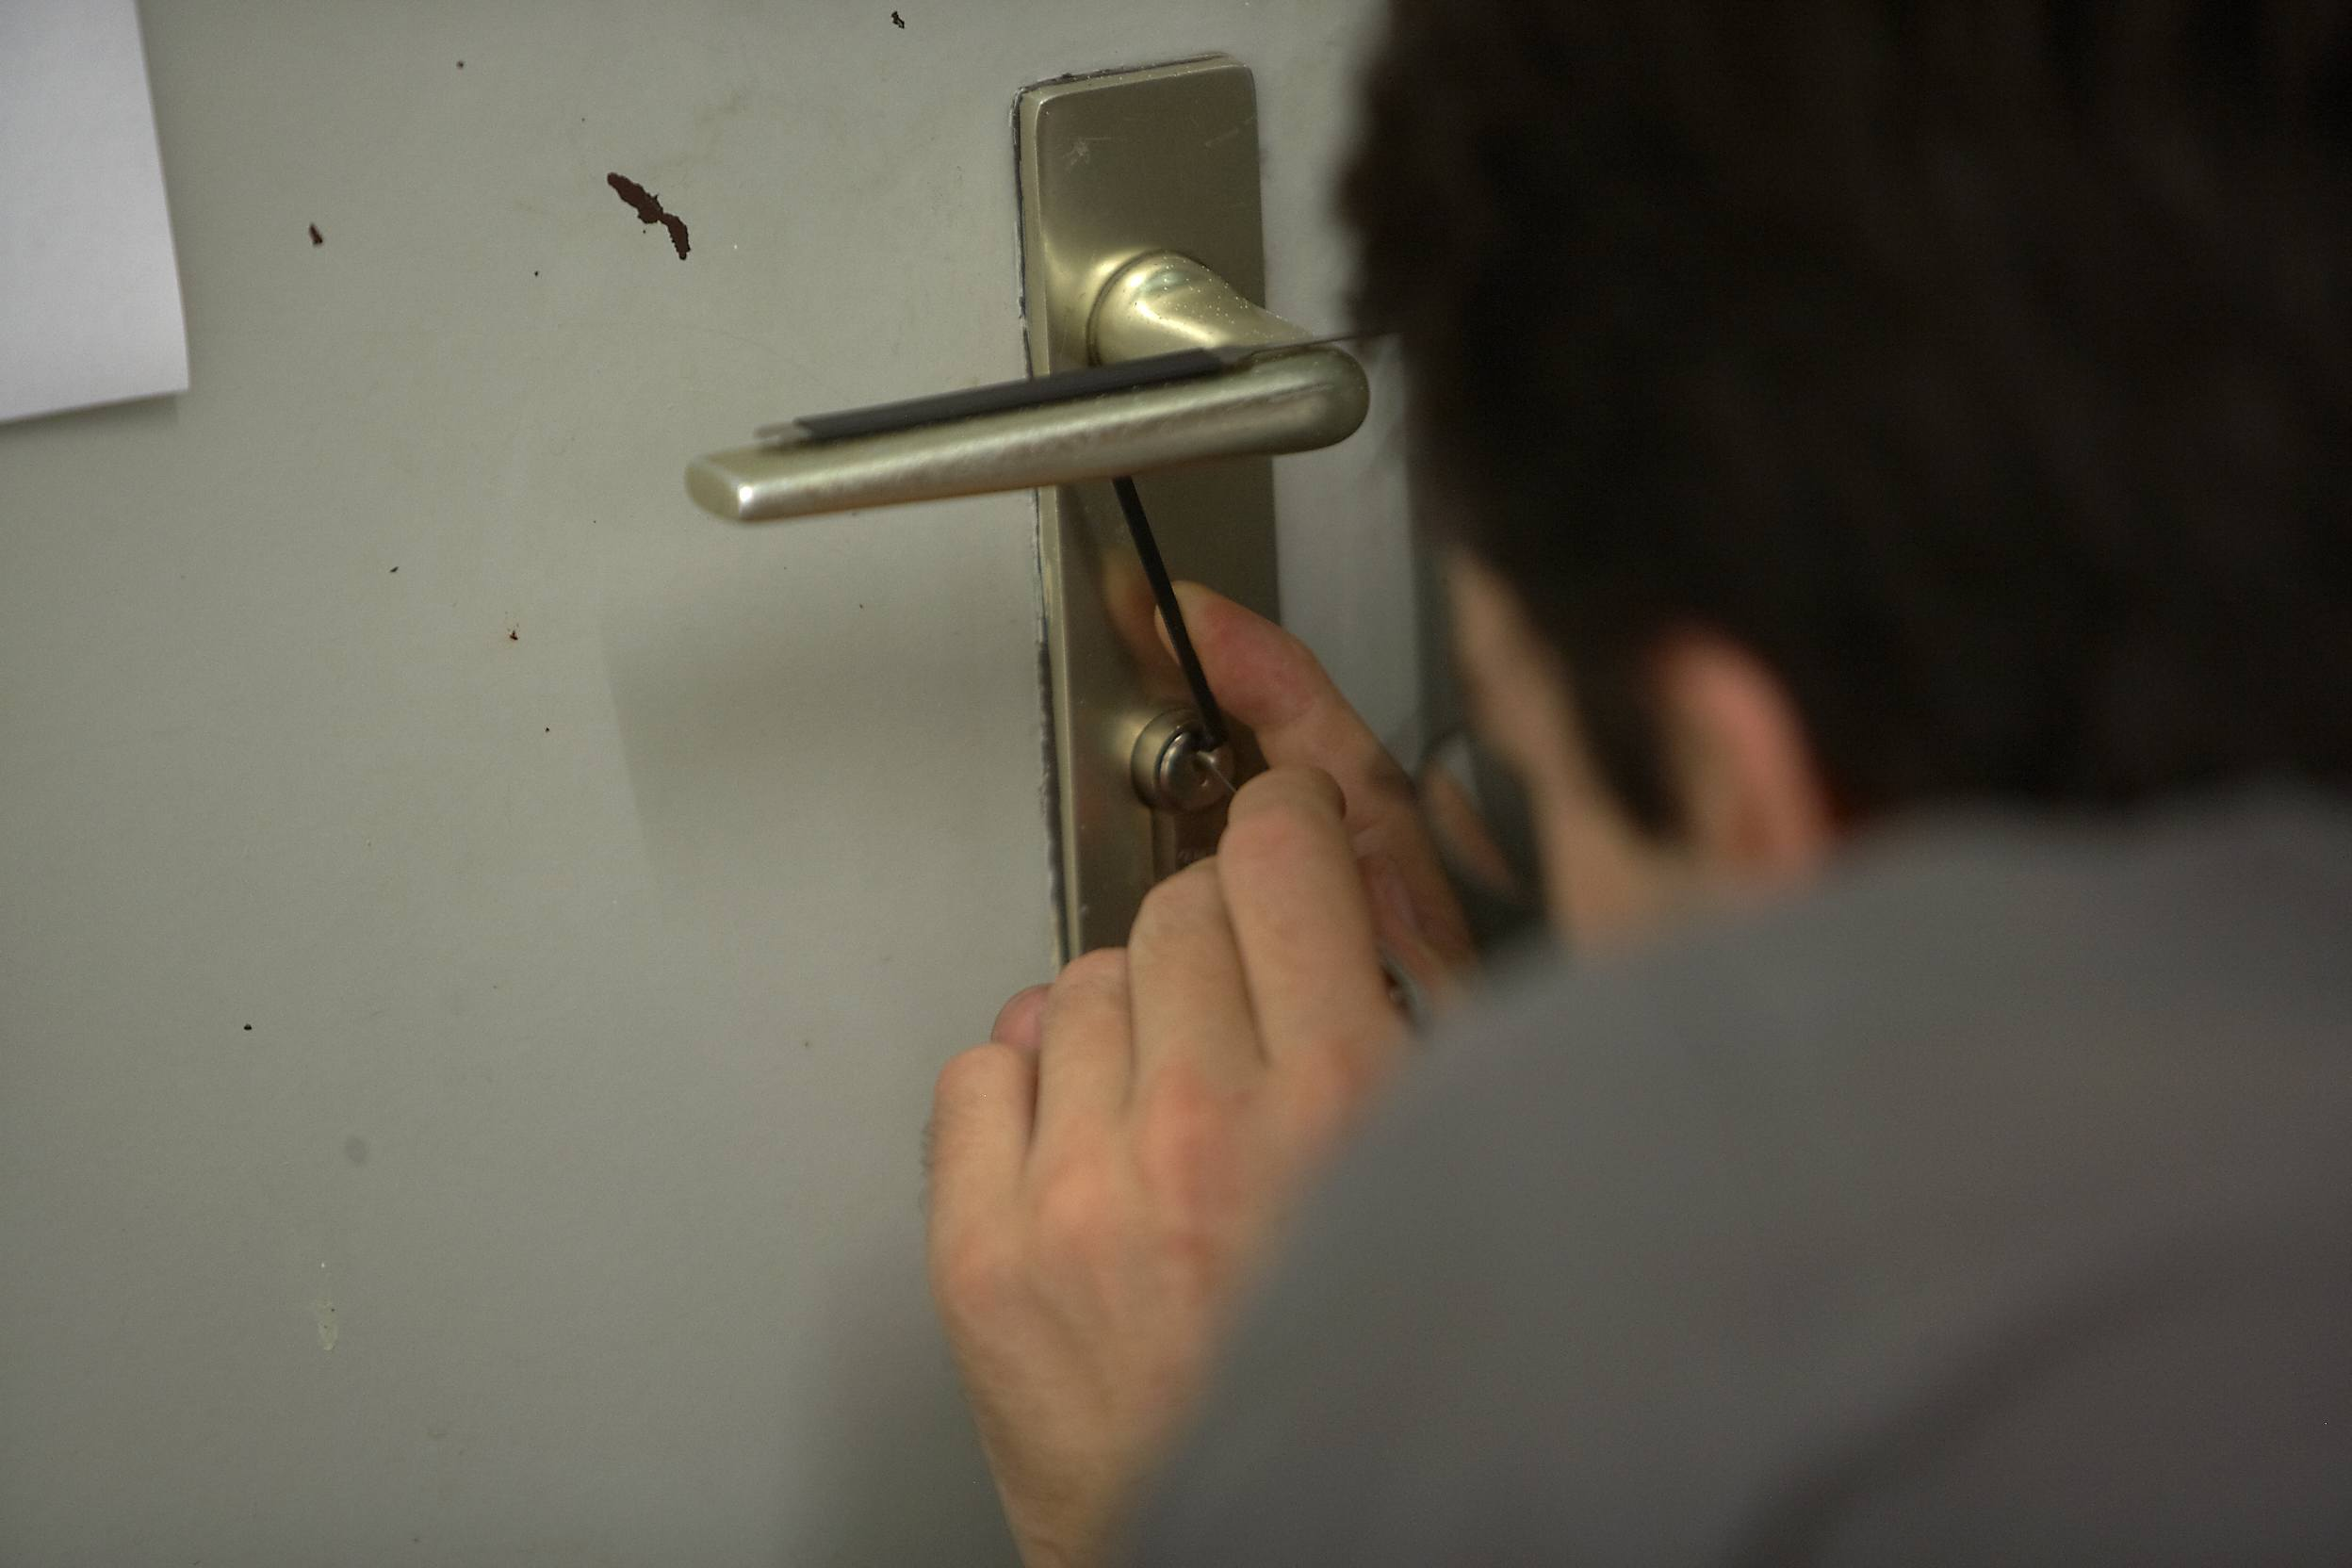
\includegraphics[height=4cm]{bilder/ipick.jpg}\\
        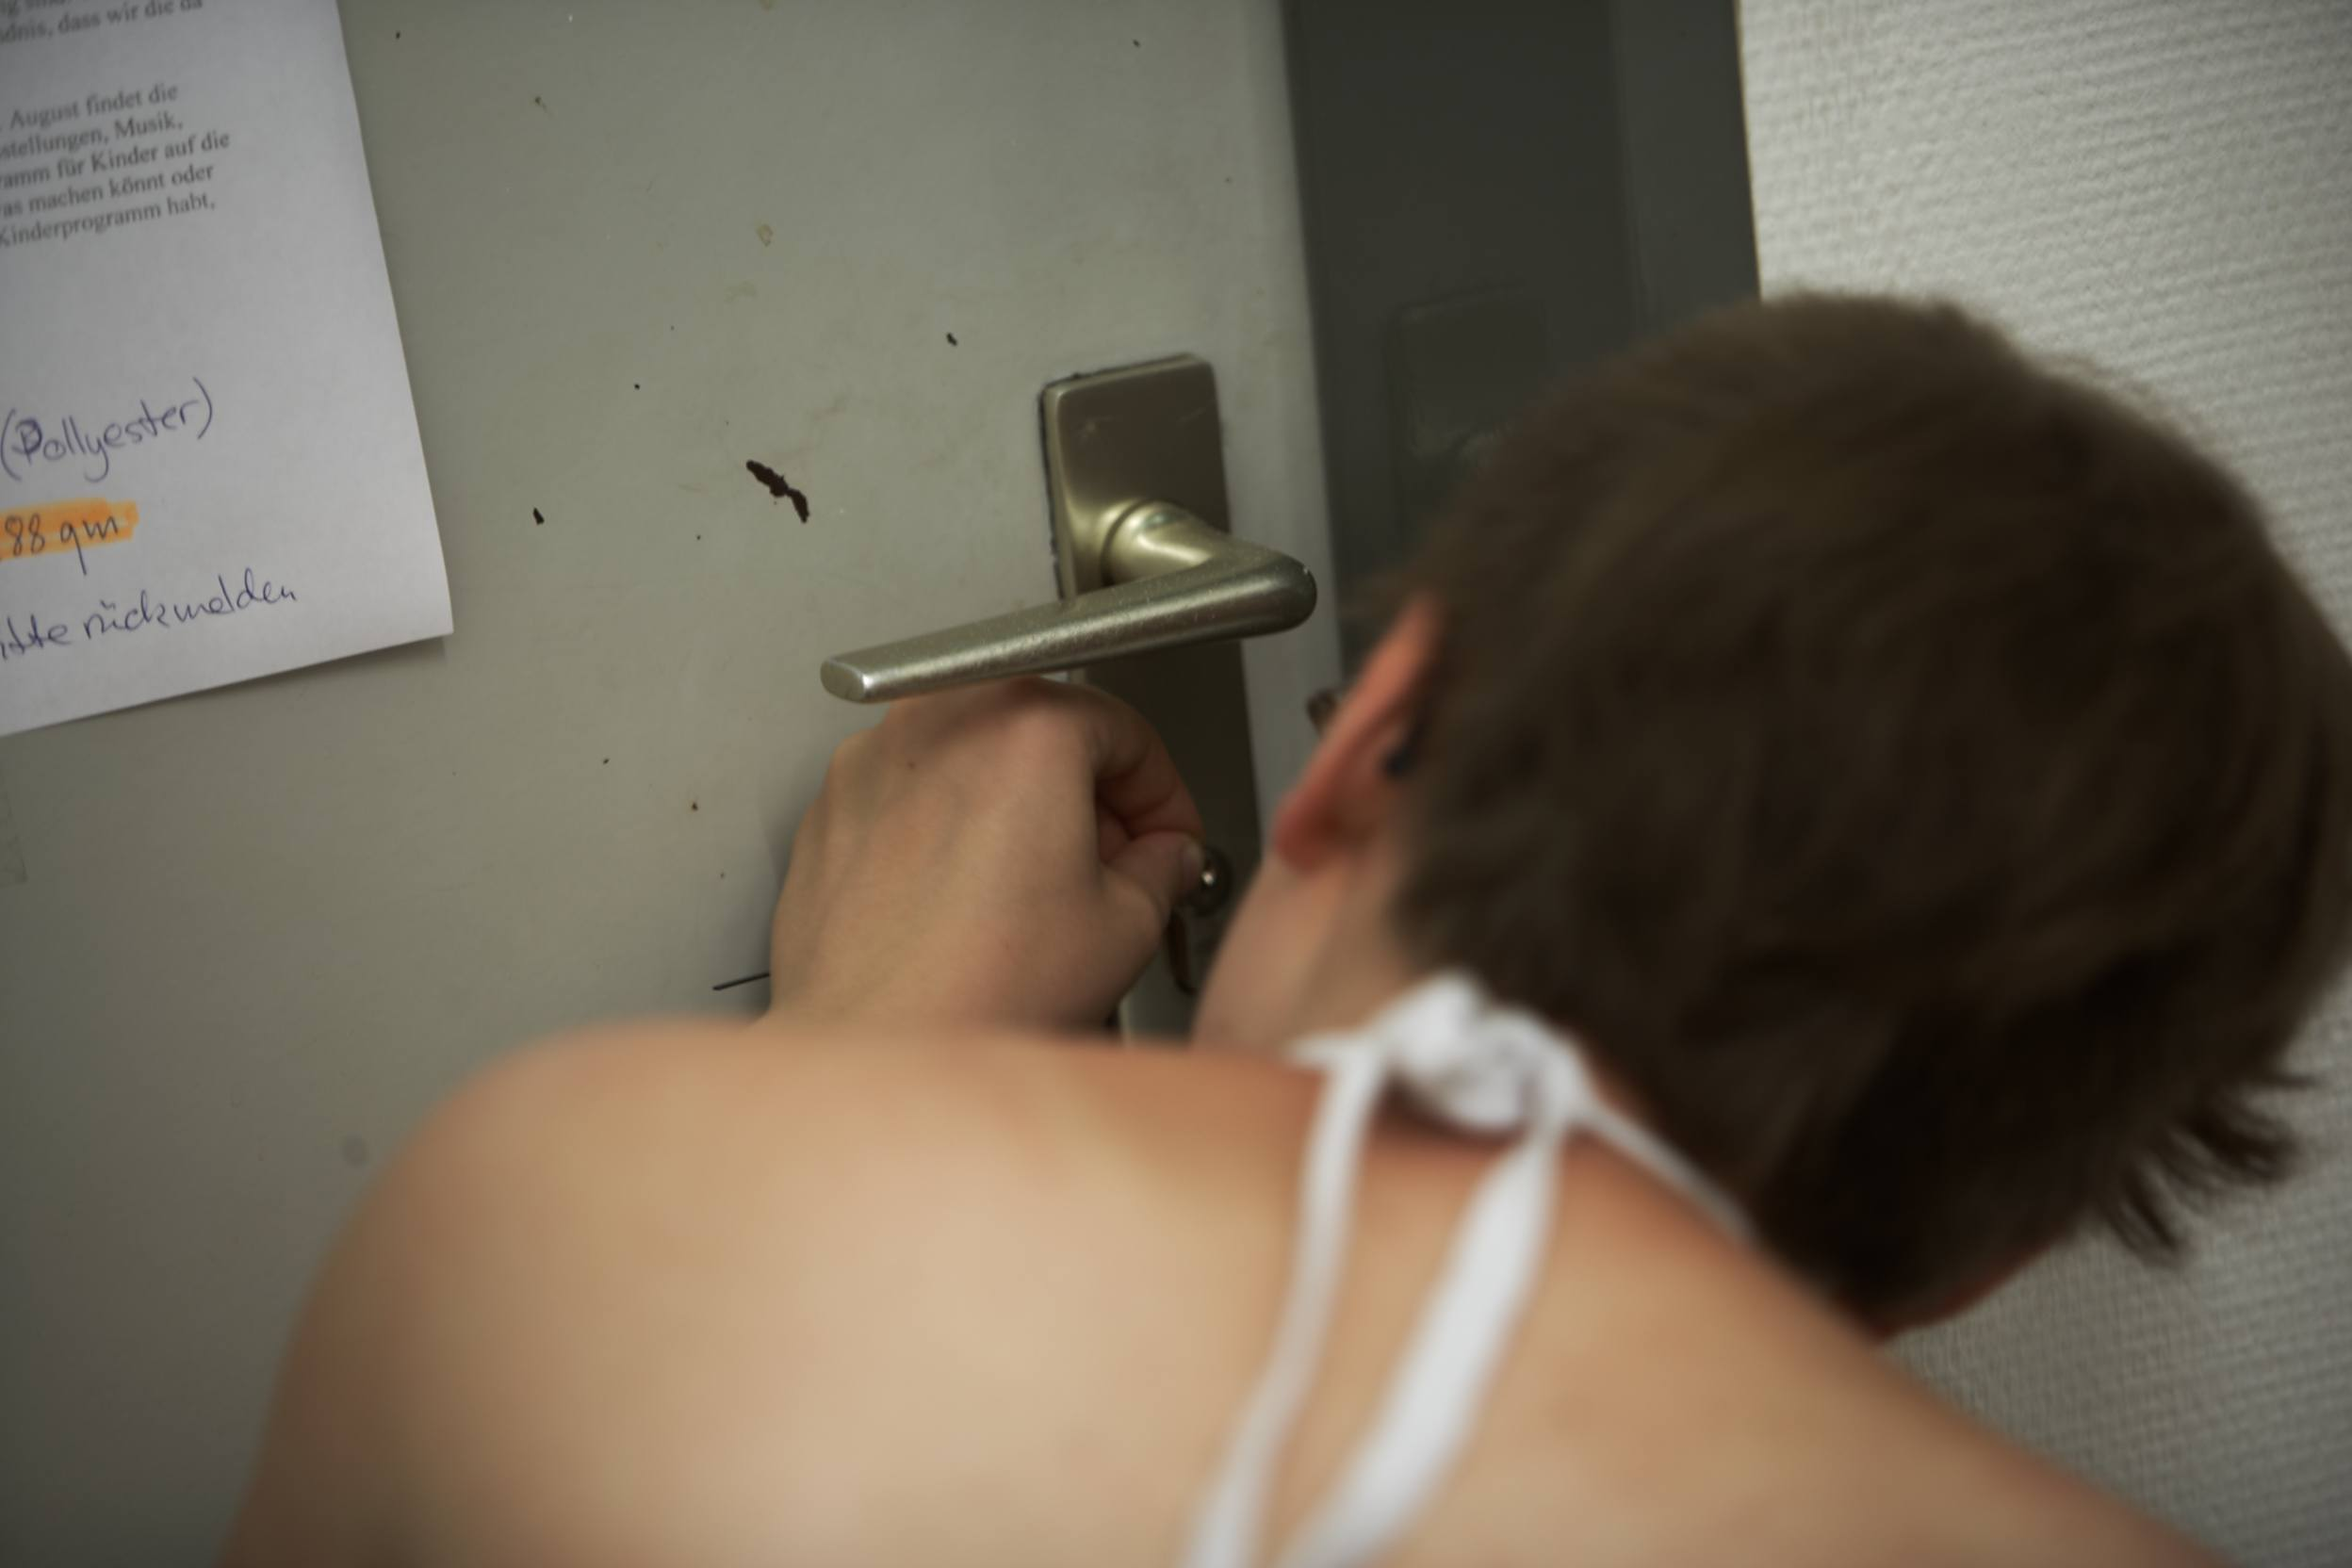
\includegraphics[height=4cm]{bilder/lpick.jpg}
    \end{column}
    \begin{column}{6cm}
        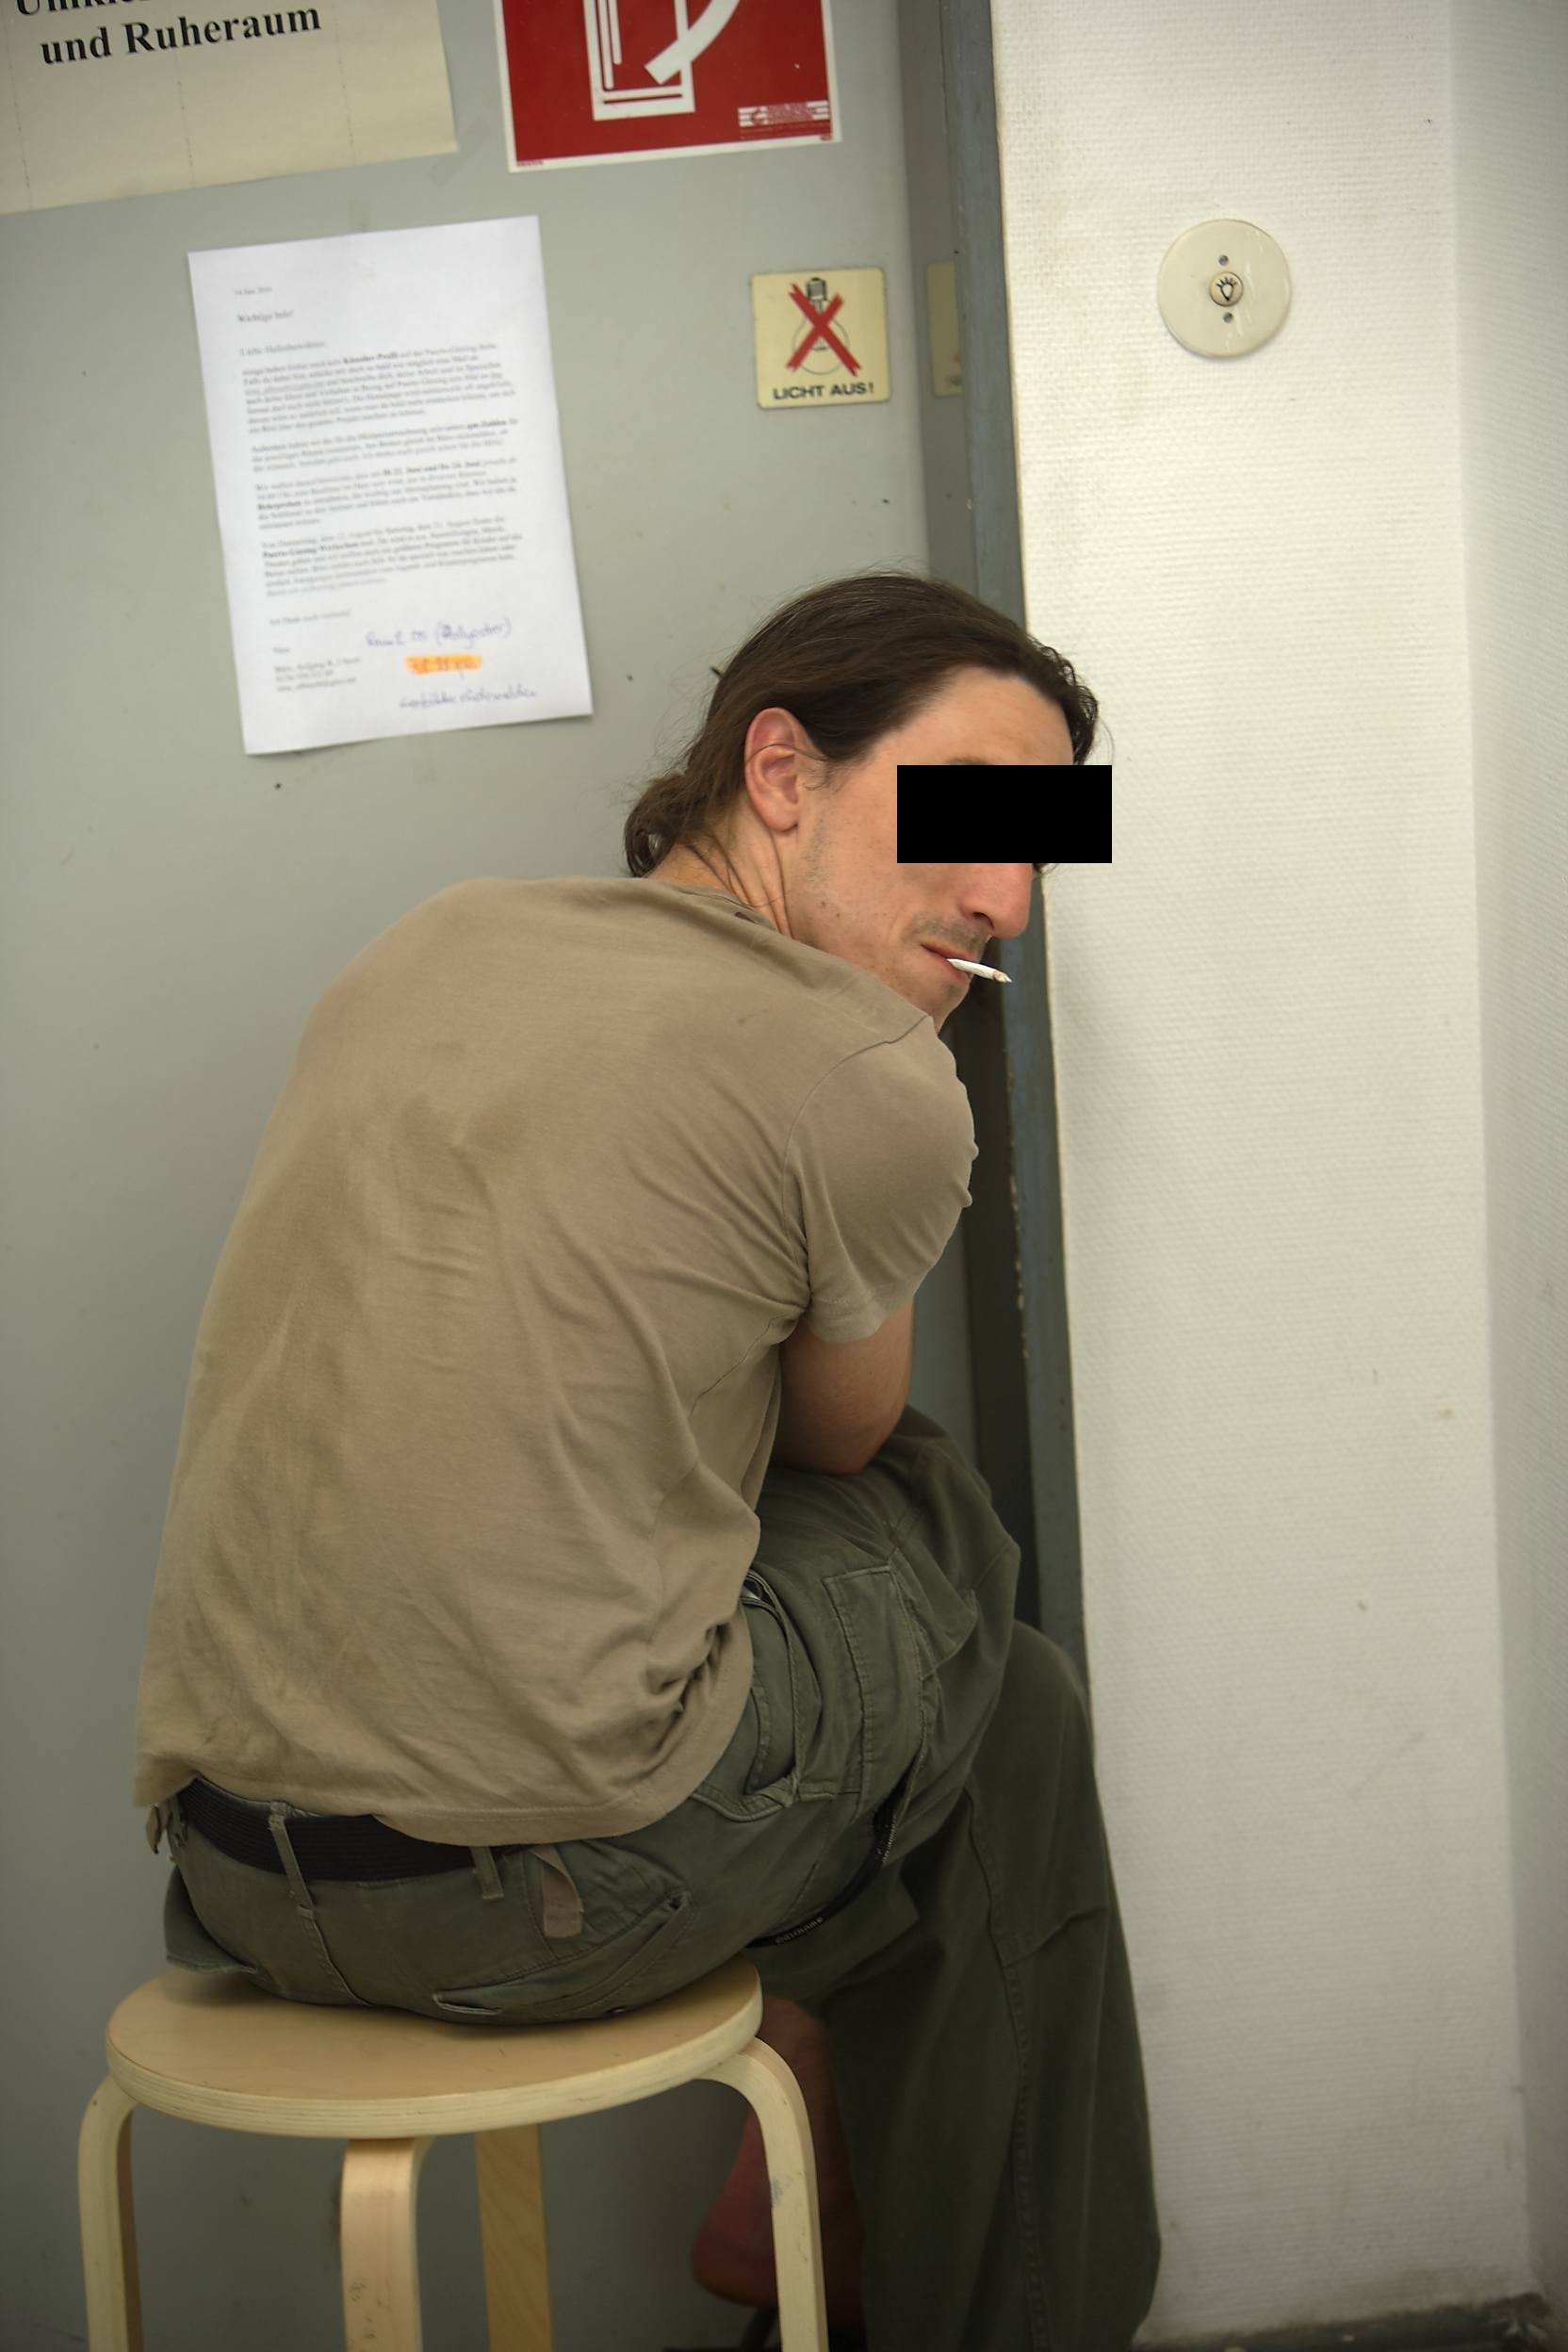
\includegraphics[height=8cm]{bilder/apick.jpg}
    \end{column}
  \end{columns}
\end{frame}
\section{Hardware}
  \begin{frame}{A lamp fit for the project}
    \begin{columns}
      \begin{column}{3.5cm}
        \begin{figure}
          \begin{center}
          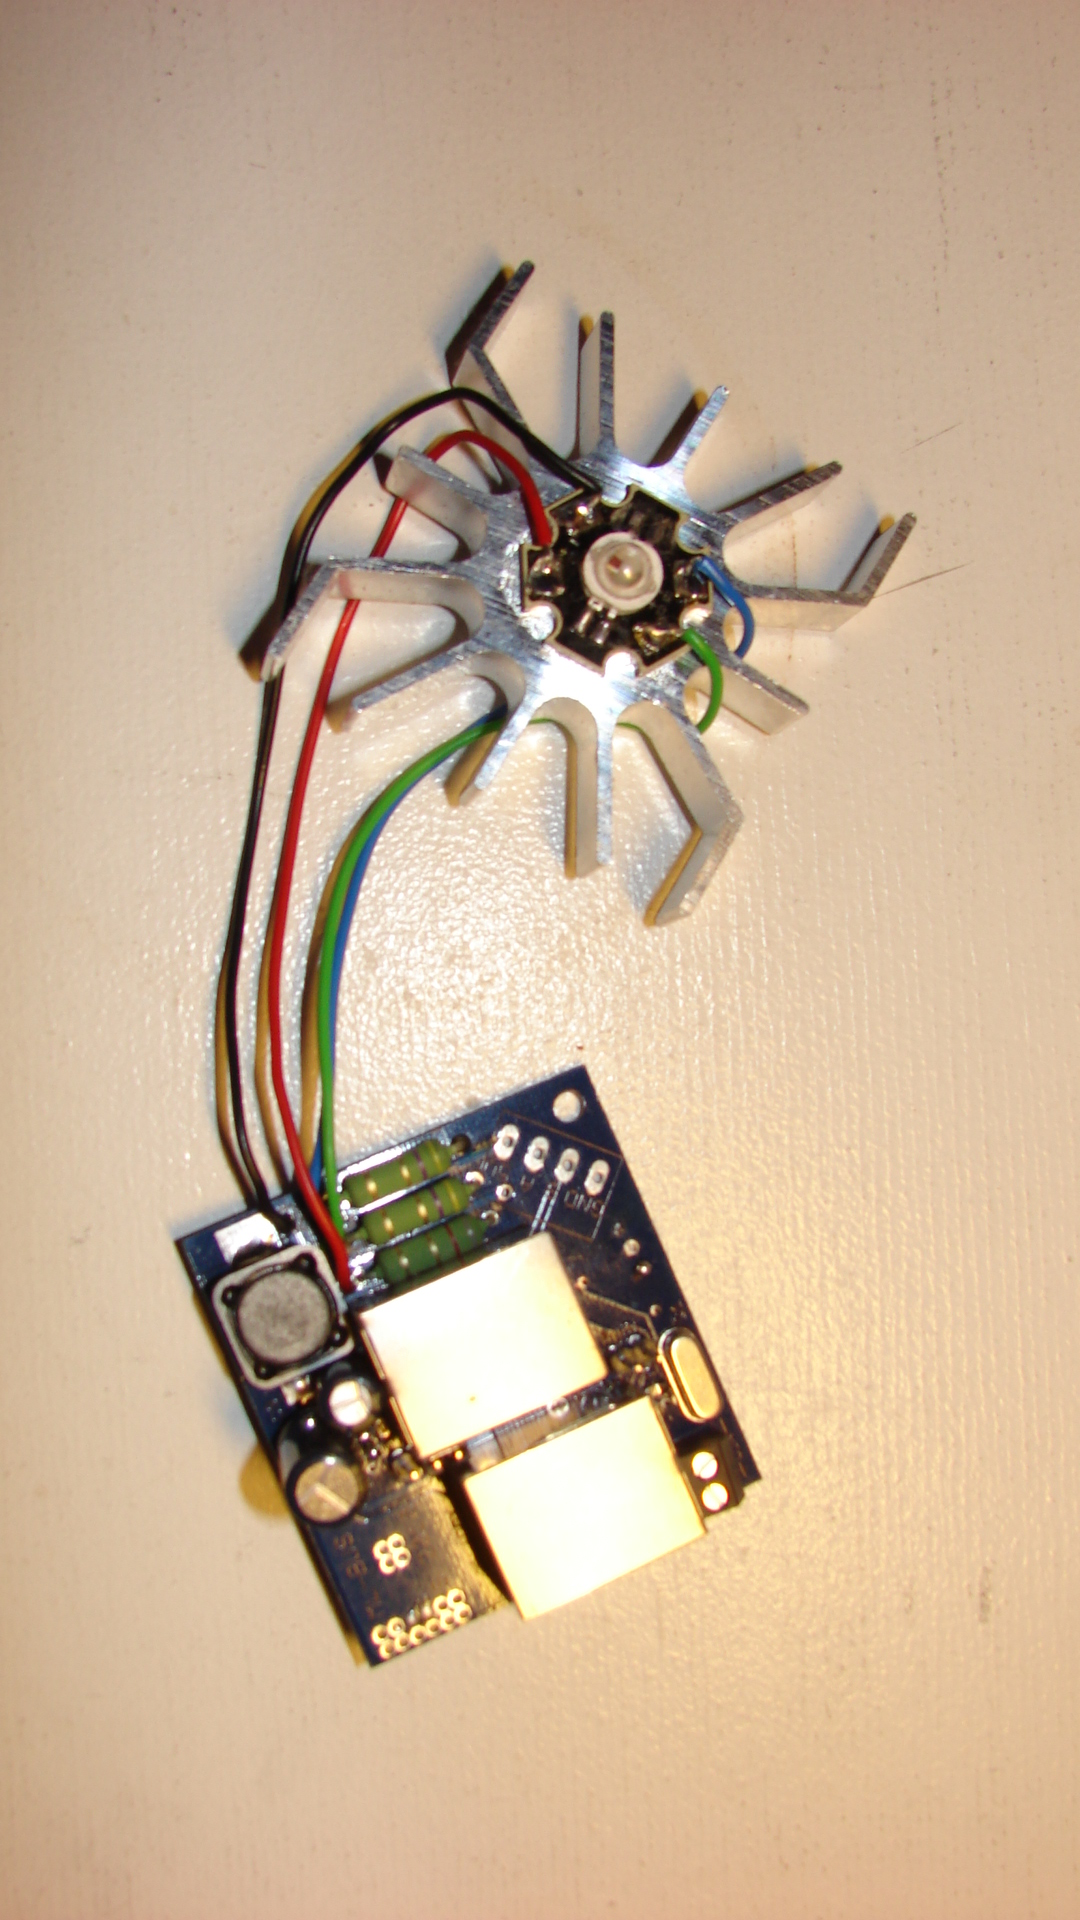
\includegraphics[width=3cm]{bilder/lampe1.JPG}
          \end{center}
        \end{figure}
      \end{column}
      \begin{column}{5cm}
        \begin{itemize}
        \item New lamp, only neccessary components
        \item Switching regulator for higher supply voltage (-> lower supply current)
        \item Ethernet connectors replace old screw terminals for faster and more stable(?) connections
        \end{itemize}
      \end{column}
      \begin{column}{3.5cm}
         \begin{figure}
          \begin{center}
          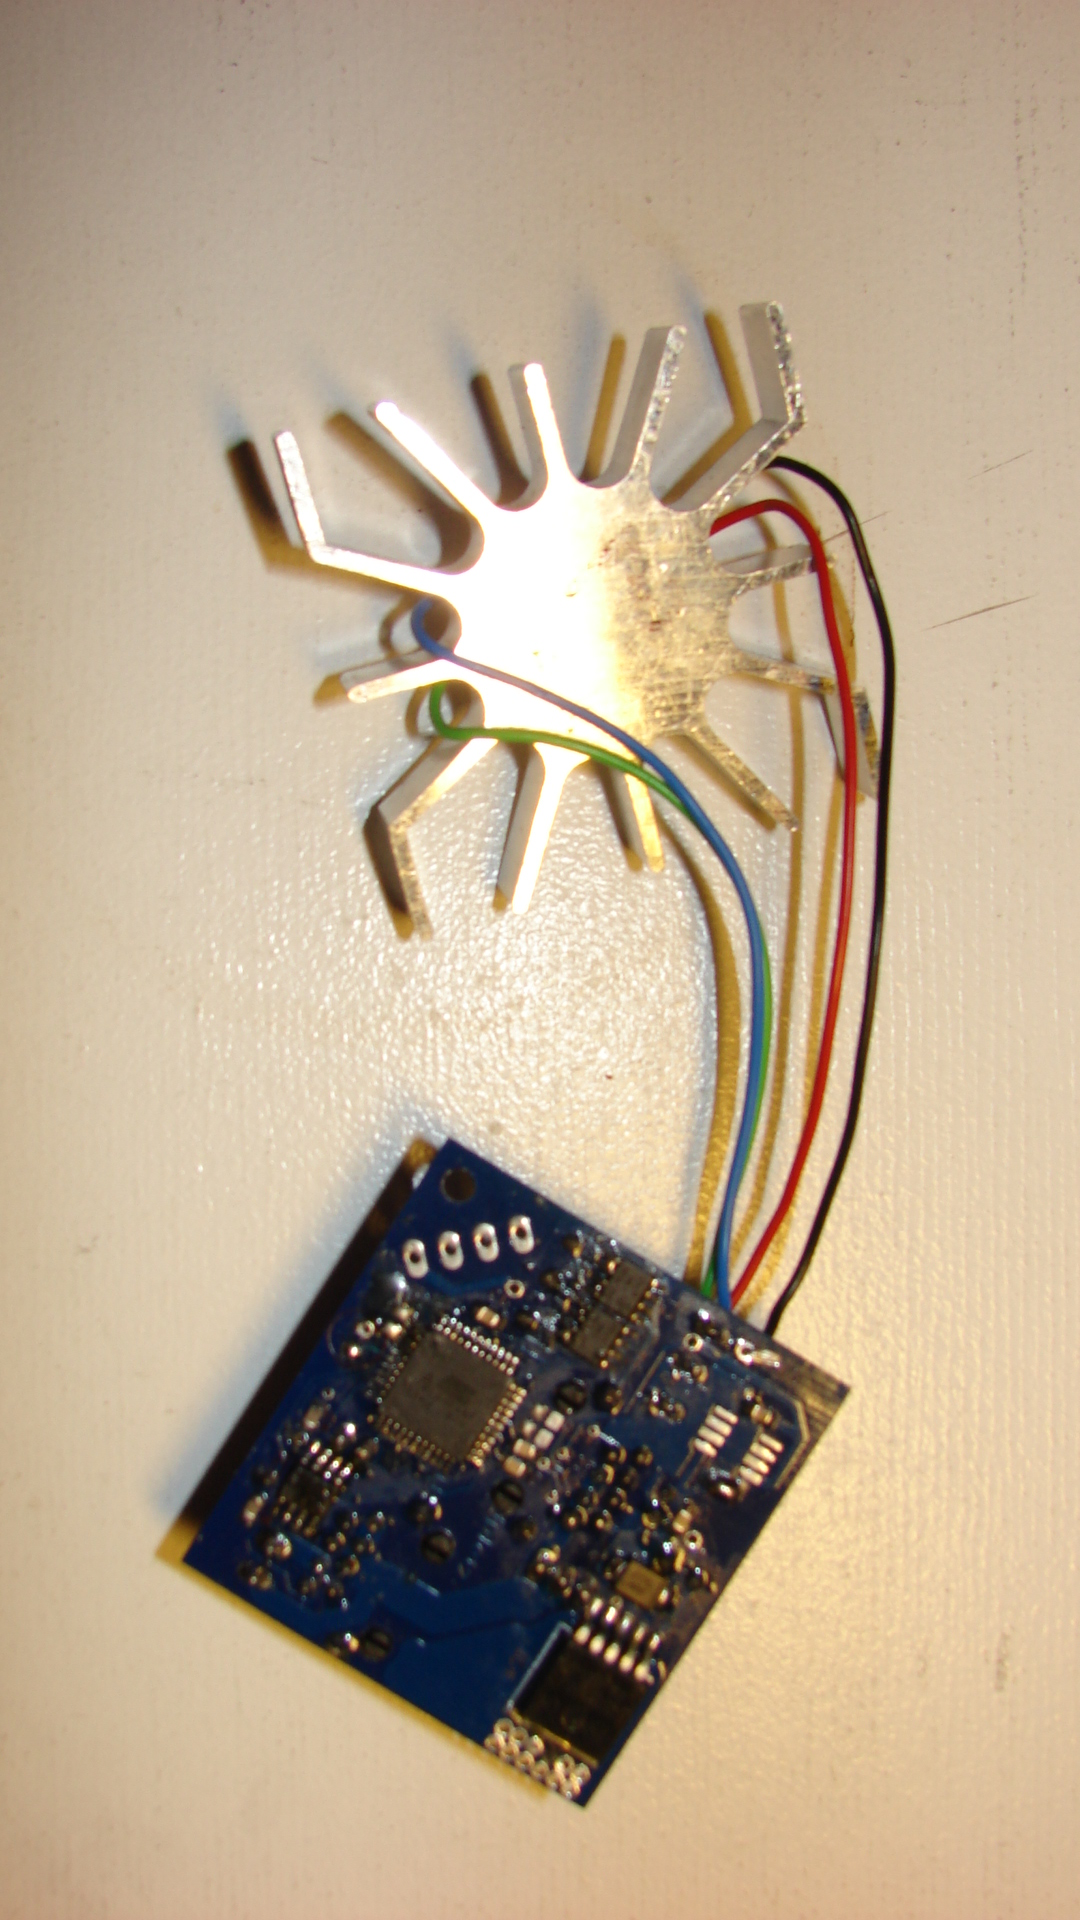
\includegraphics[width=3cm]{bilder/lampe2.JPG}
          \end{center}
        \end{figure}
     \end{column}
    \end{columns}
  \end{frame}
  \begin{frame}{The lamp - Outline}
    \begin{figure}
    \begin{center}
    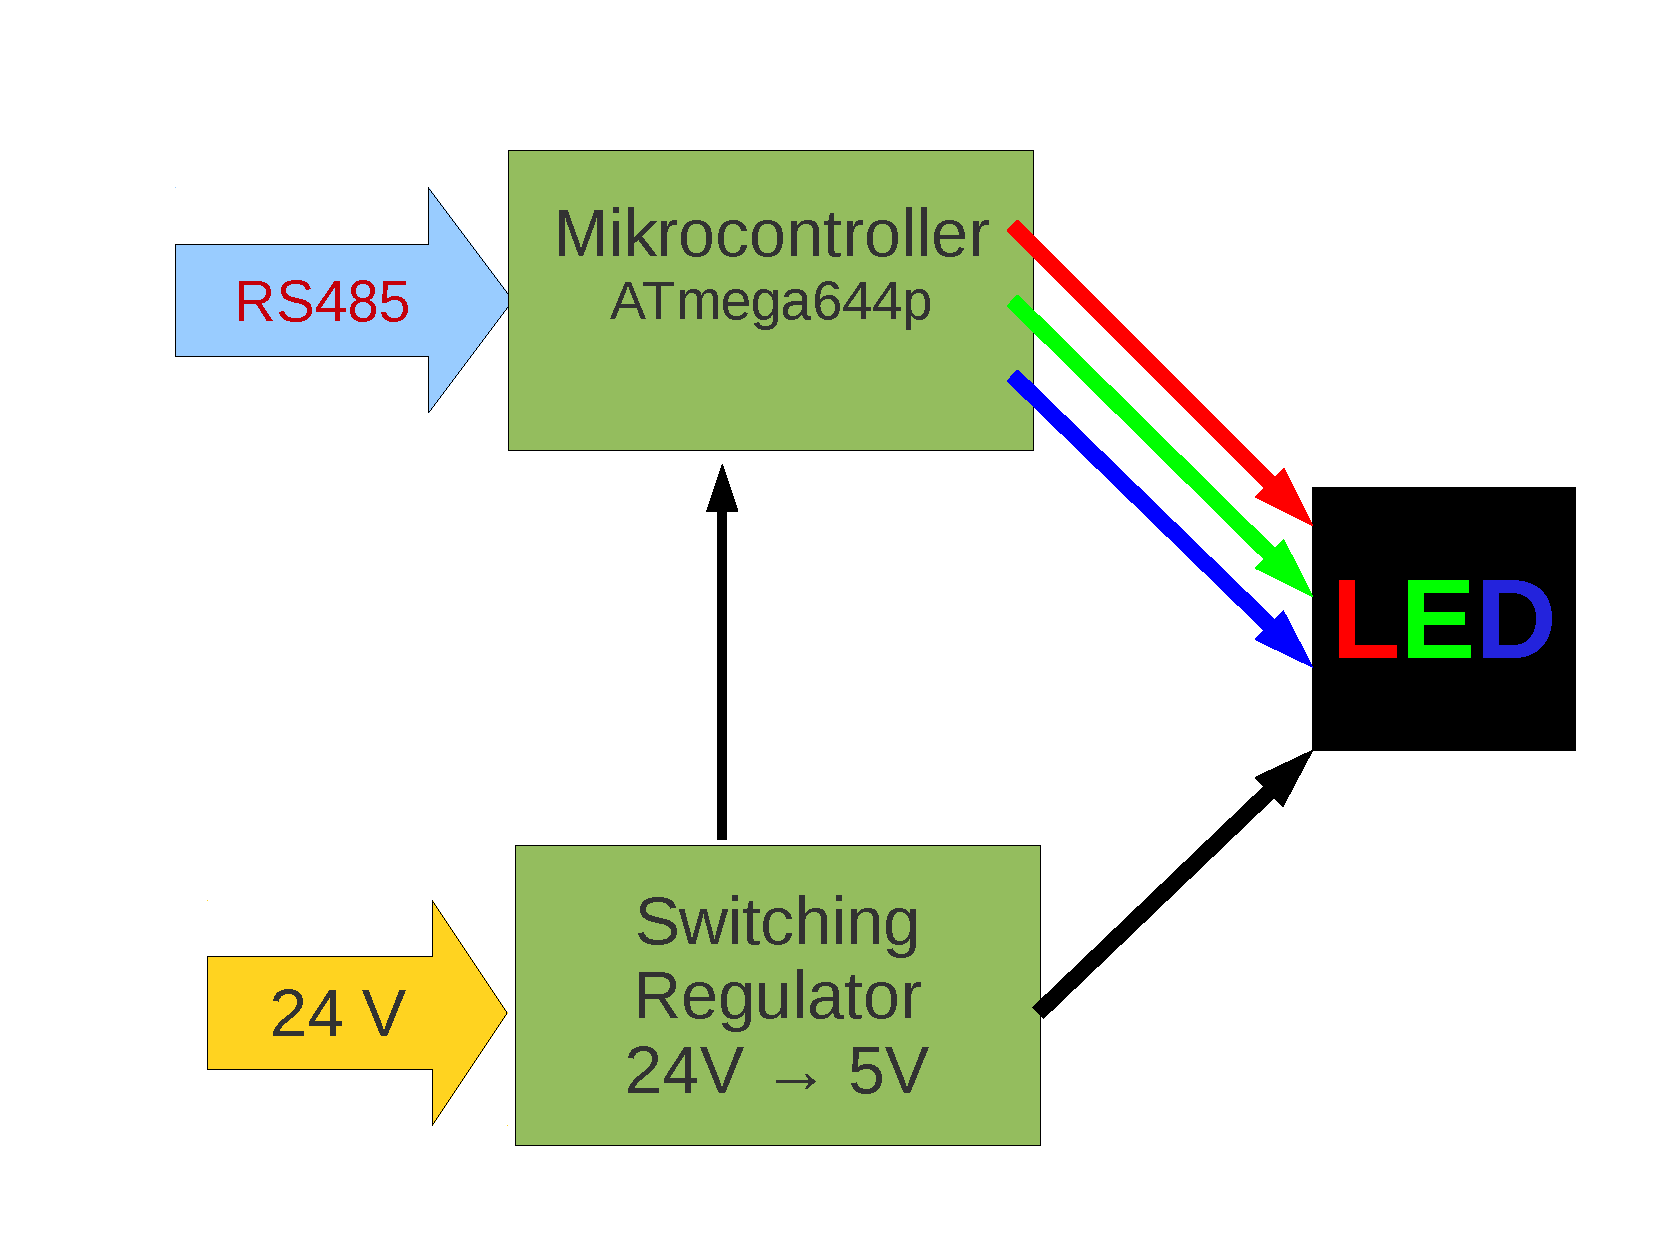
\includegraphics[width=9cm]{bilder/led_12v_rs485.pdf}
    \end{center}
    \end{figure}
  \end{frame}
  \begin{frame}{Power Supply}
  At 24V supply voltage one power supply unit suffices for 16 lamps.
  \begin{columns}
    \begin{column}{4cm}
     \begin{block}{ Puerto Giesing}
     Two supply units are used to supply the 24 lamps of one row
     \end{block}
     \begin{block}{27c3}
     One supply unit is used for the 16 lamps of one row
     \end{block}
    \end{column}
    \begin{column}{7cm}
    \begin{figure}
    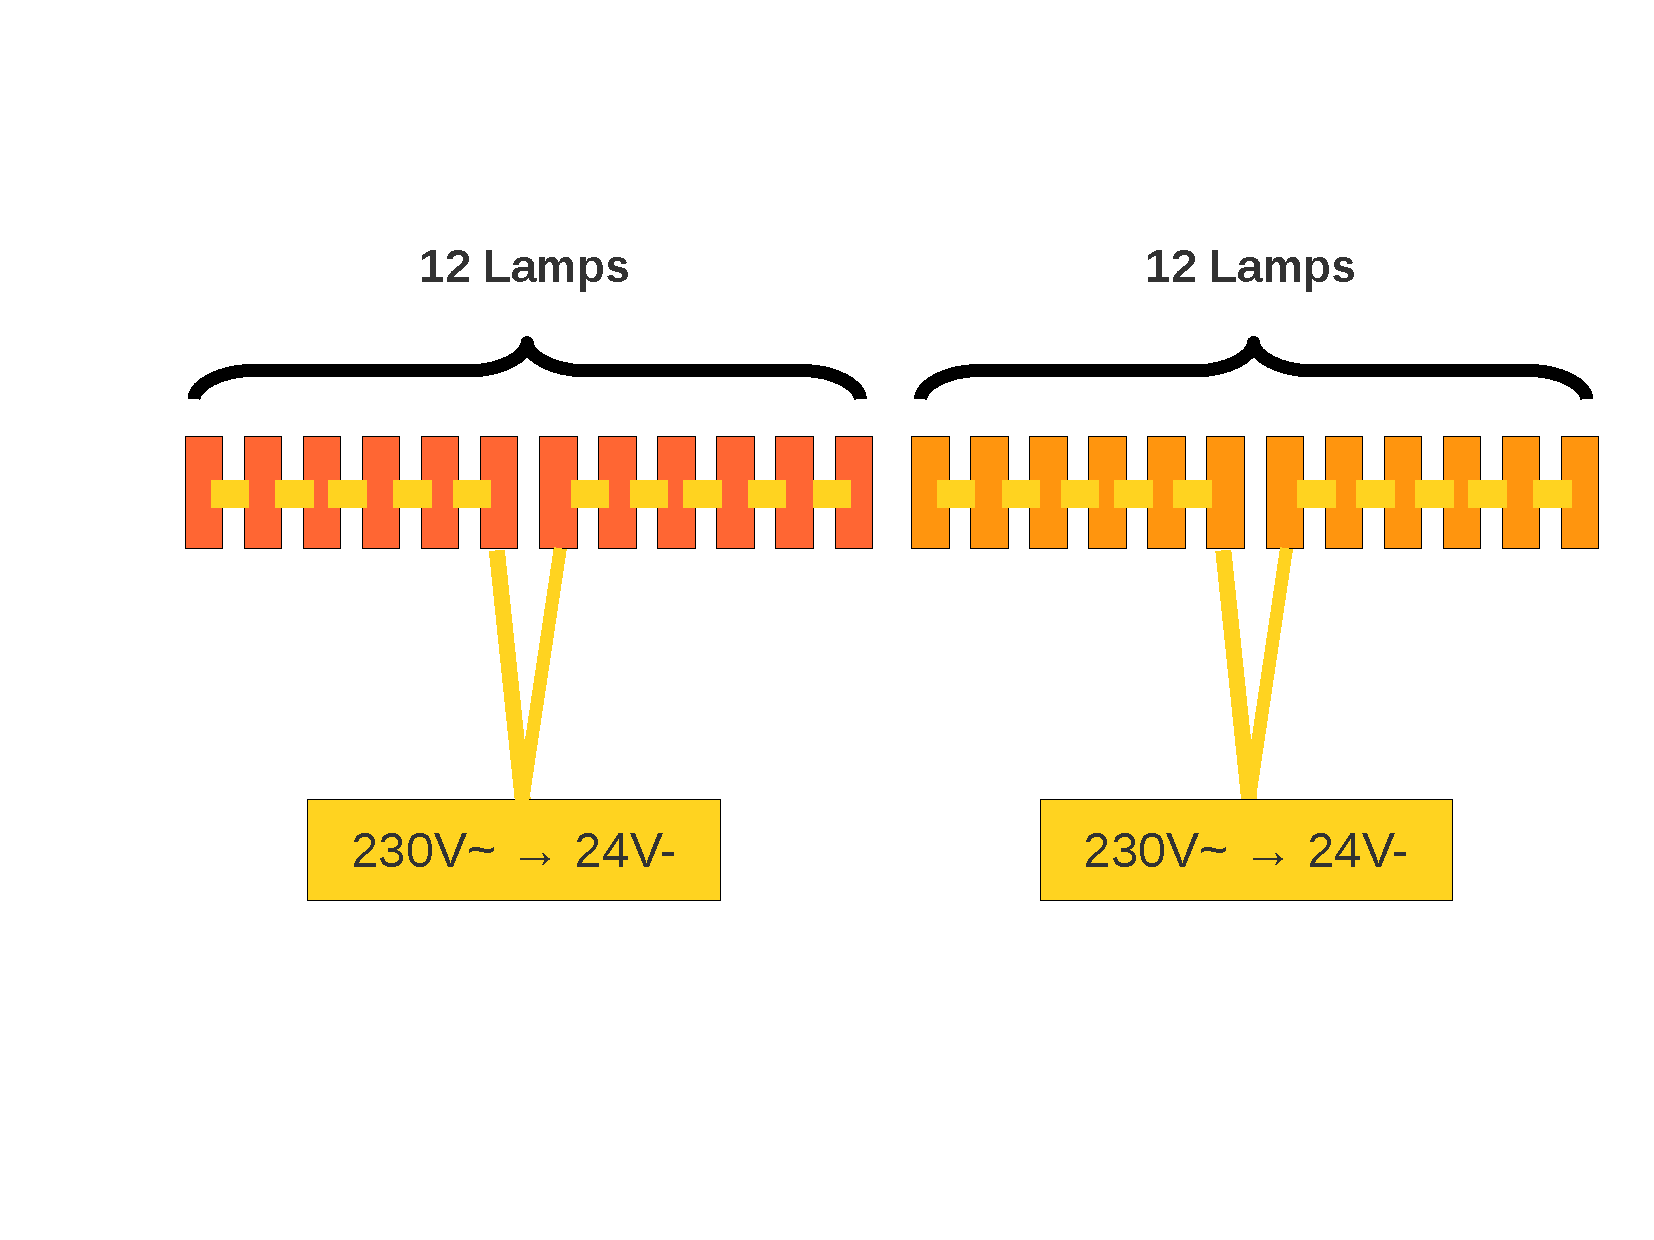
\includegraphics[width=7cm, clip, trim= 2.5cm 4.6cm 0.5cm 4cm]{bilder/12lampen.pdf}
    \end{figure}
    \end{column}
  \end{columns}
  \end{frame}
  \begin{frame}{Data Exchange}
    \begin{itemize}
      \item Data exchange over regular ethernet cables
      \item 3 conductor pairs reserved for power supply
      \item Remaining one used for data
    \end{itemize}
      \begin{figure}
        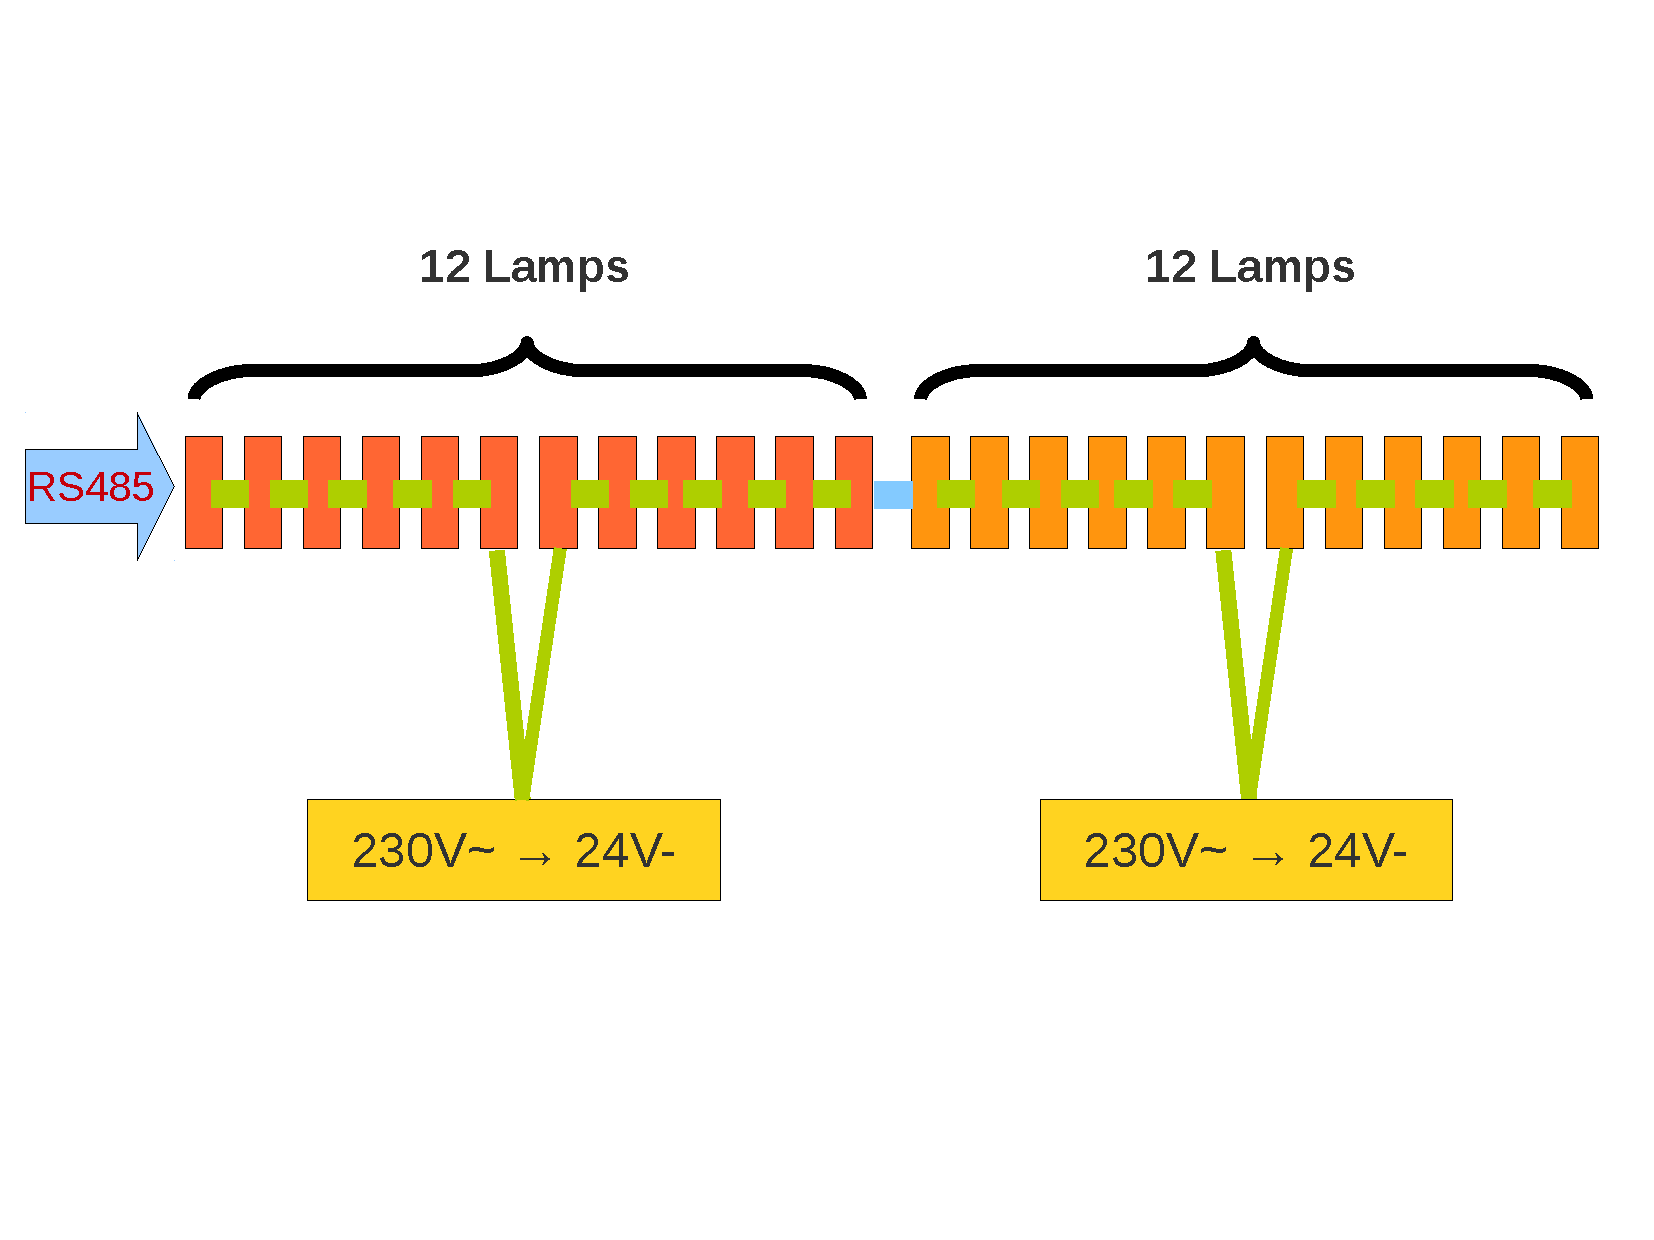
\includegraphics[width=8cm, clip, trim= 0cm 4.6cm 0.5cm 4cm]{bilder/12lampen_rs485.pdf}
        \caption{Puerto Giesing}
      \end{figure}
  \end{frame}
  \begin{frame}{RS485}
    \begin{columns}
       \begin{column}{6cm}
        \begin{figure}
        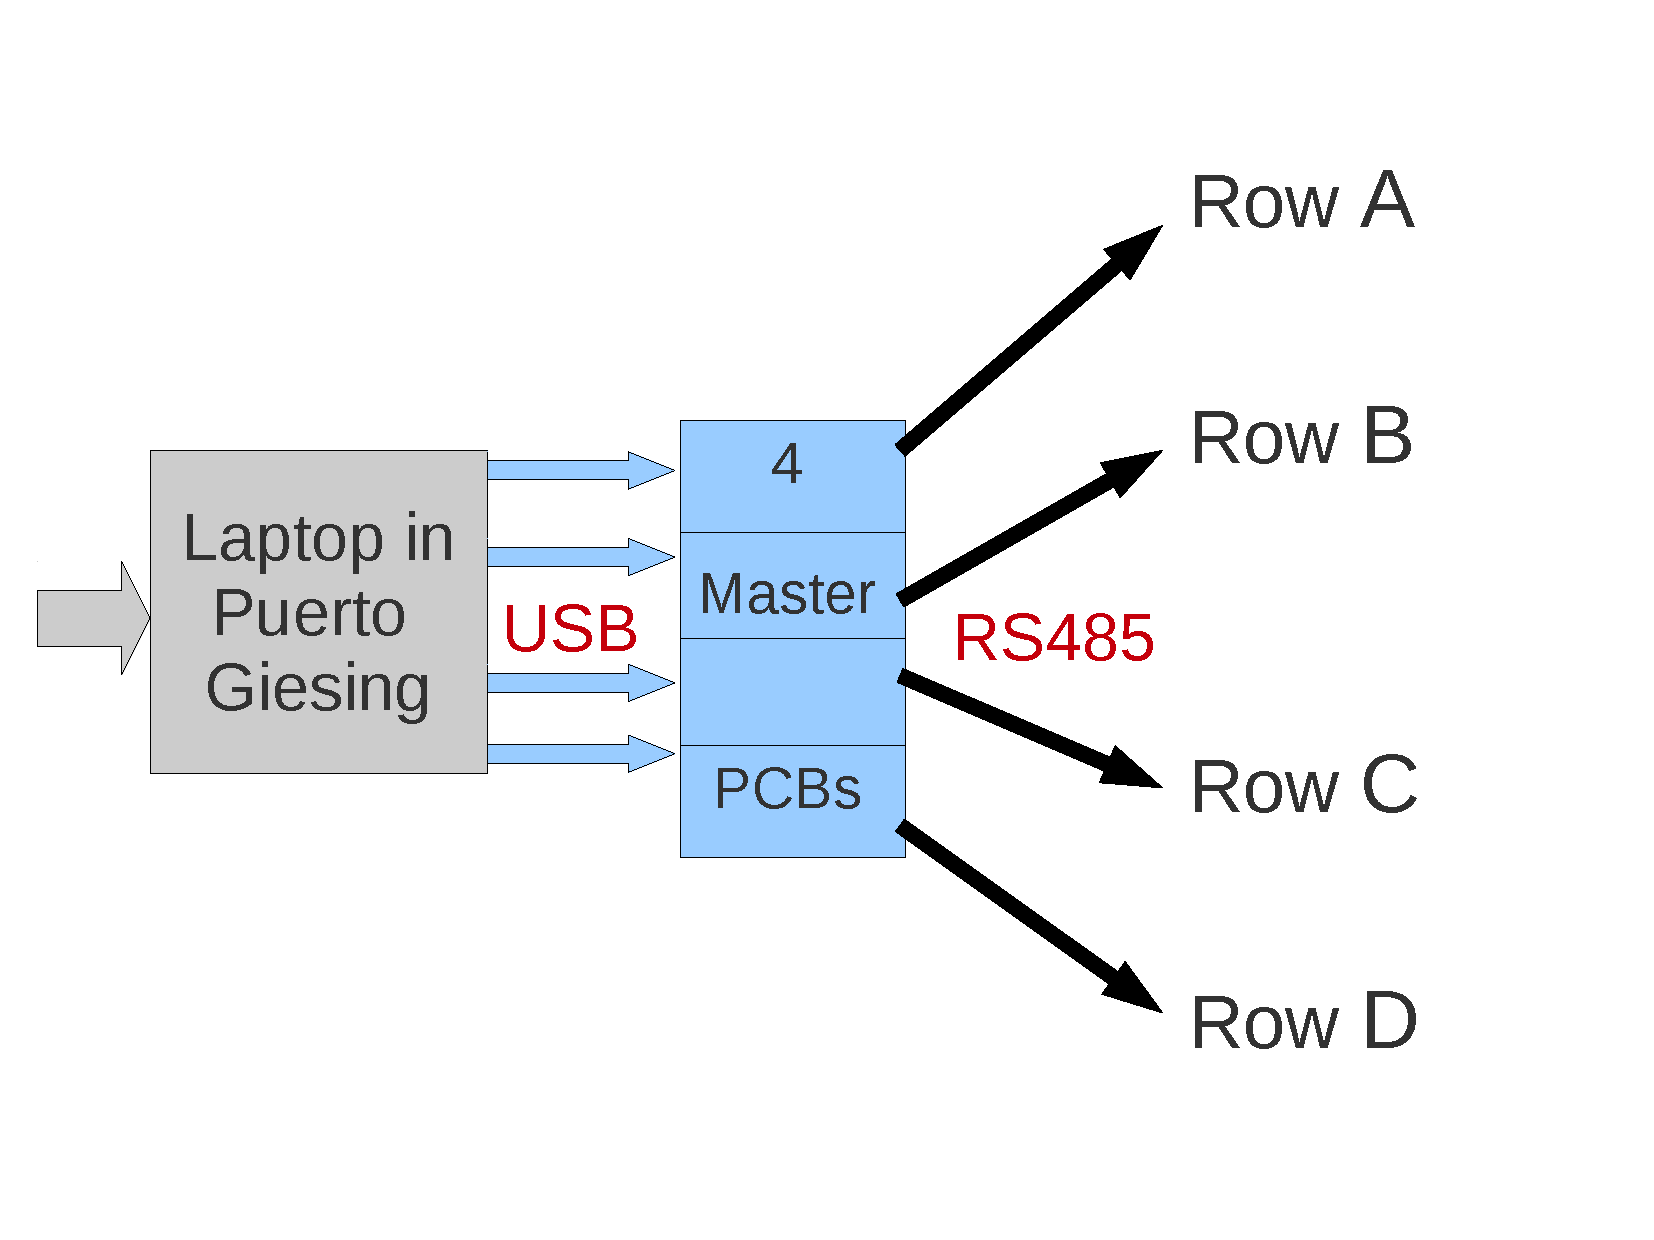
\includegraphics[width=6cm, clip, trim= 1cm 3cm 4cm 2.5cm]{bilder/laptop.pdf}
        \end{figure}
      \end{column}
     \begin{column}{5cm}
        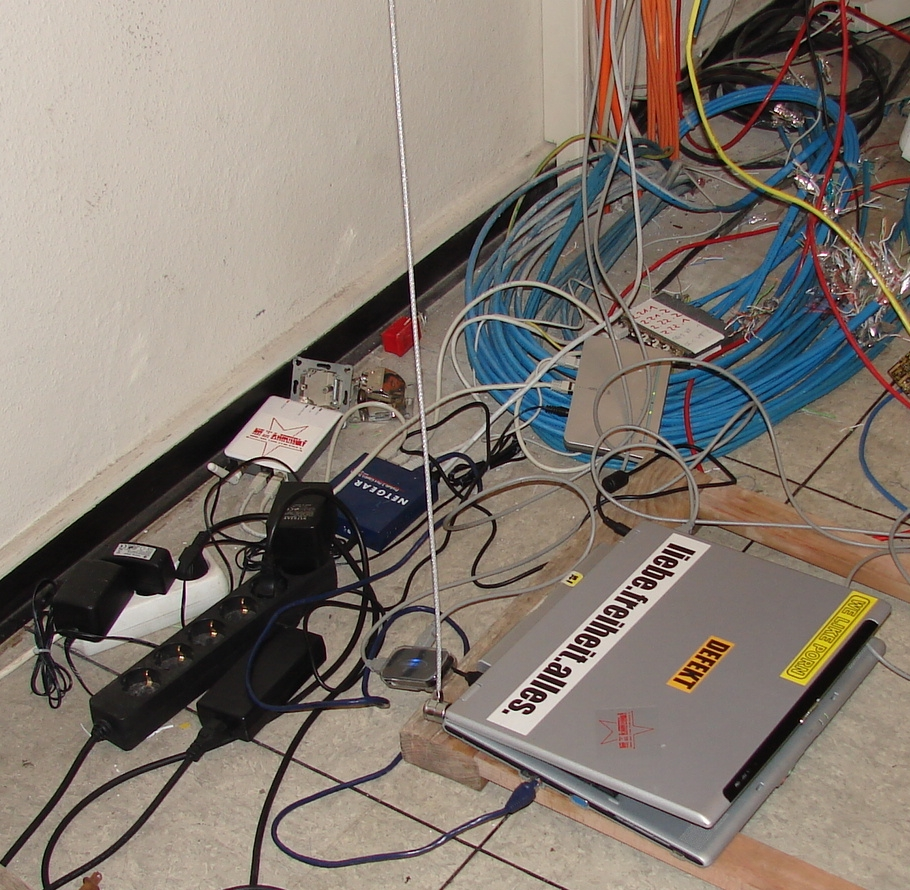
\includegraphics[width=5cm, clip, trim= 0cm 0cm 0cm 0cm]{bilder/laptop.jpg}
     \end{column}
   \end{columns}
   \begin{columns}
     \begin{column}{9cm}
       \begin{block}{RS485}
        \begin{itemize}
        \item \small Versatile communication standard
        \item \small Connects several devices in bus structure
        \item \small Communication over long distances
        \end{itemize}
       \end{block}
     \end{column}
   \end{columns}
  \end{frame}

\section{Software}

\begin{frame}{Software Components}

    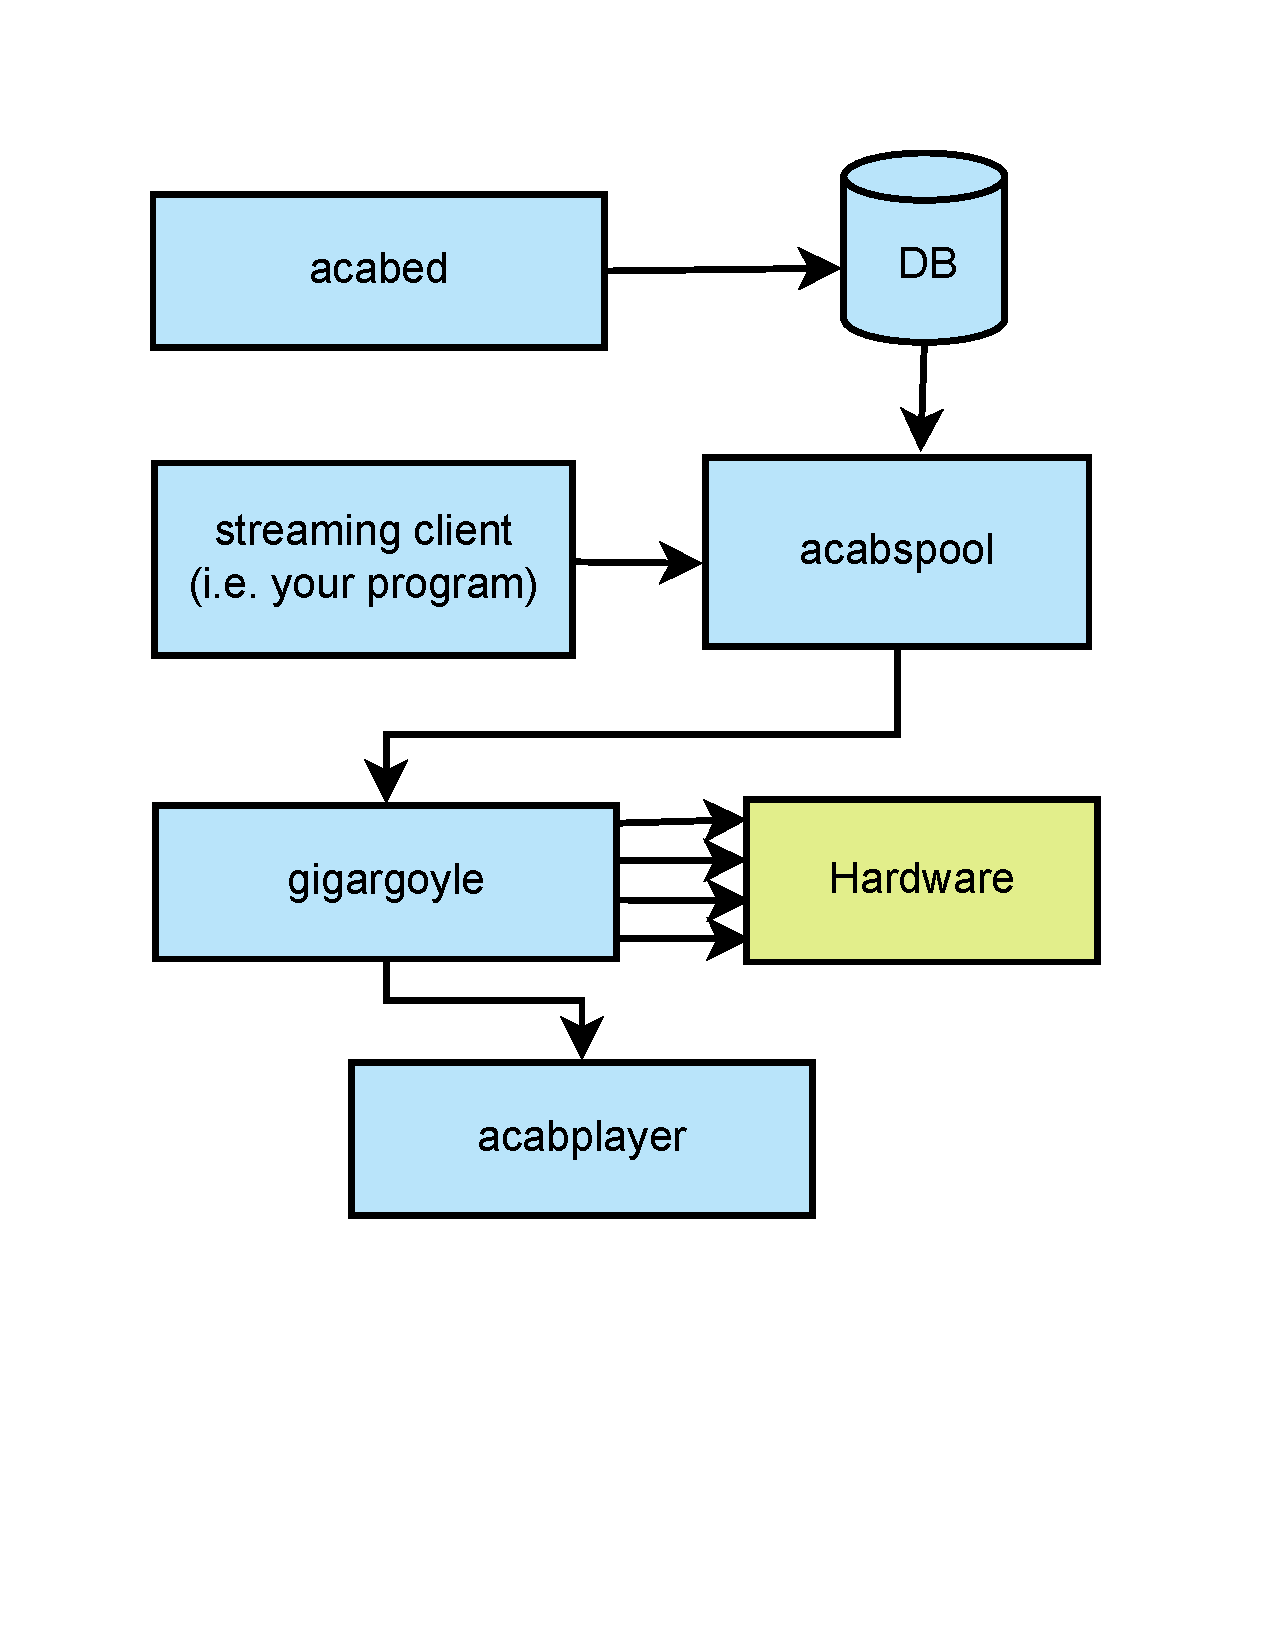
\includegraphics[height=\paperheight/1.1]{bilder/software.pdf}

\end{frame}

\begin{frame}{Software Components (2)}
    \begin{columns}
	\begin{column}{5cm}
	    \begin{block}{acabed}
		\begin{itemize}
		    \item Webeditor
		    \item Python (Django)
		    \item JavaScript (Mootools)
		\end{itemize}
	    \end{block}
	    \begin{block}{Streaming Clients}
		\begin{itemize}
		    \item Roll your own interactive live streams
		    \item Python Library available
		\end{itemize}
	    \end{block}
	    \begin{block}{acabplayer}
		\begin{itemize}
		    \item Live Viewer
		    \item C, SDL
		\end{itemize}
	    \end{block}
	\end{column}
	\begin{column}{5cm}
	    \begin{block}{acabspool}
		\begin{itemize}
			\item Queueing/Streaming Manager
			\item Python
			\item Manages streaming from
			    database or direct streamers
		\end{itemize}
	    \end{block}
	    \begin{block}{gigargoyle}
		\begin{itemize}
		    \item Display ``Driver''
		    \item C
		    \item Gets raw animations, puts them on the screen
		\end{itemize}
	    \end{block}
	\end{column}
    \end{columns}
\end{frame}

\begin{frame}{acabed}

    acabed live demonstration

\end{frame}

\section{Putting it all together}

\begin{frame}{Putting it all together}
  \begin{columns}
    \begin{column}{10cm}
      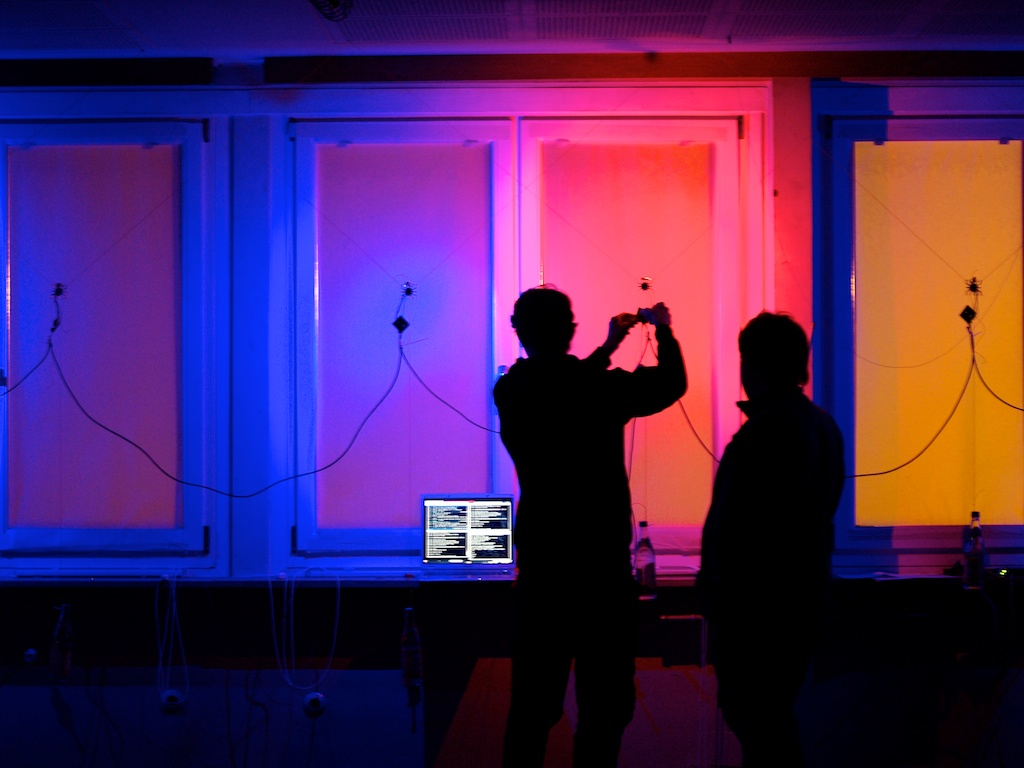
\includegraphics[width=10cm]{bilder/tests.jpg}
    \end{column}
  \end{columns}
\end{frame}

\begin{frame}{Putting it all together}
  \begin{columns}
    \begin{column}{5cm}
      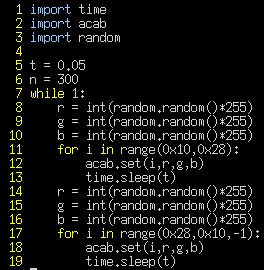
\includegraphics[width=5cm]{bilder/fill.png}
    \end{column}
    \begin{column}{5cm}
      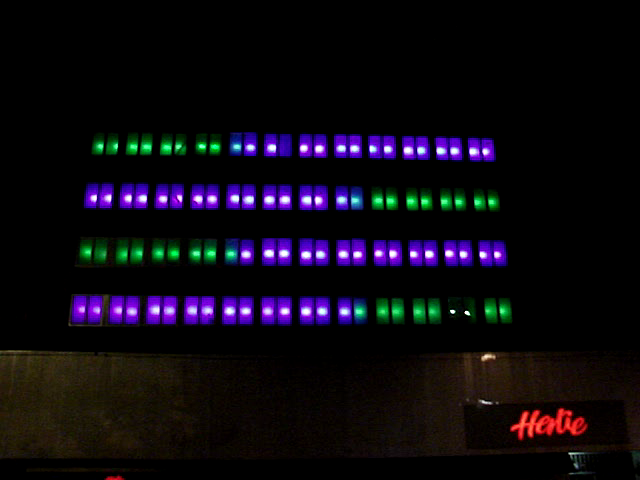
\includegraphics[width=5.5cm]{bilder/fail.png}
    \end{column}
  \end{columns}
\end{frame}

\begin{frame}{Putting it all together}
  \begin{columns}
    \begin{column}{10cm}
      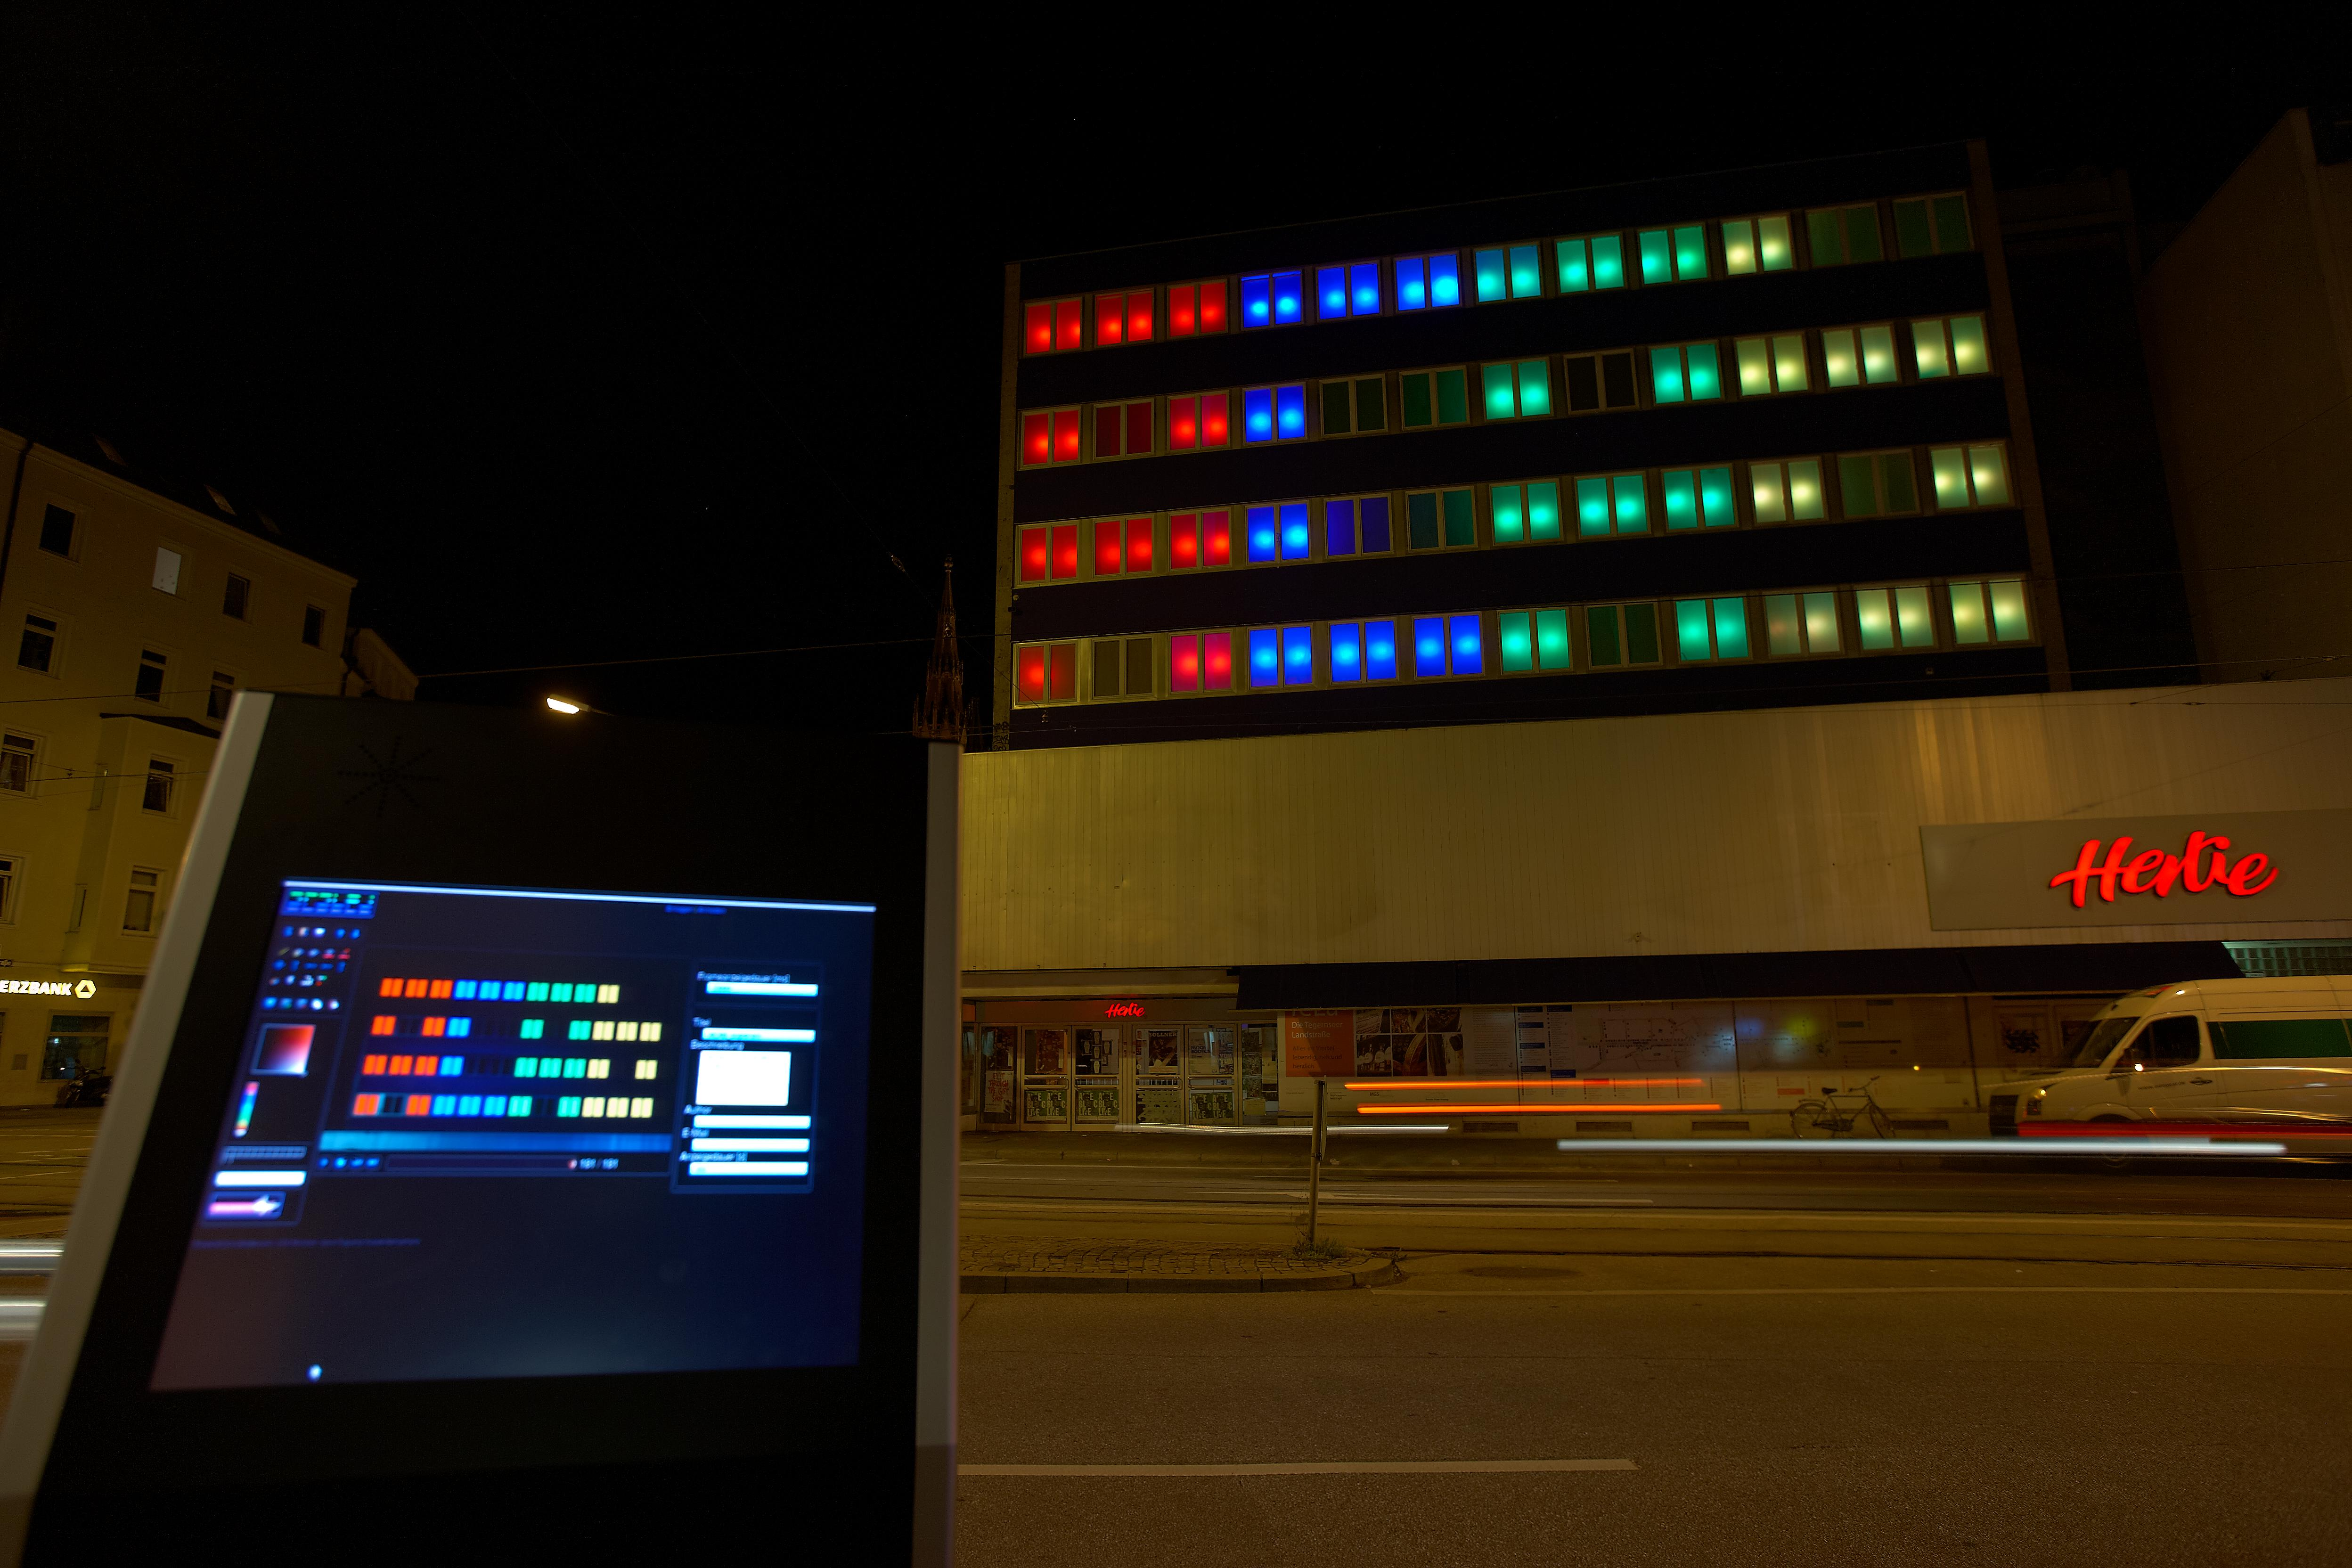
\includegraphics[width=10cm]{bilder/terminal.jpg}
    \end{column}
  \end{columns}
\end{frame}

\begin{frame}{Interaction}
    \begin{block}{Touch-Terminal}
	\begin{itemize}
	    \item Passersby could create animations on touch screen
		terminal with acabed
	    \item Donation
	\end{itemize}
    \end{block}

    \begin{block}{SMS}
	\begin{itemize}
	    \item Text Message could trigger animation play
	    \item \texttt{play ID}
	\end{itemize}
    \end{block}
    
    \begin{block}{blubbtris by Aquarium}
	\begin{itemize}
	    \item Live Tetris Game
	    \item indepentently developed
	\end{itemize}
    \end{block}
\end{frame}


\section{acab@27c3}
  \begin{frame}{acab@27c3}
      \begin{block}{Setup}
            \begin{itemize}
               \item Plastic boxes instead of windows
               \item 6 rows with 16 boxes (makes text is possible)
               \item 6 busses, every bus with 16 lamps powered by one power supply
            \end{itemize}
	\end{block}
	\begin{block}{Play with me!}
	    \begin{itemize}
		\item Create animations with our webeditor:
		    \url{http://http://81.163.62.30/}
		\item Code games, visualizations with our Python client
		    library: \url{https://github.com/muccc/abracadabra}
	    \end{itemize}
	\end{block}
  \end{frame}
\section{acab anywhere}
  \begin{frame}{acab anywhere}
  \begin{columns}
    \begin{column}{5cm}
      \begin{block}{Software}
        \begin{itemize}
        \item Mapping of lampIDs possible to any combination of lines and columns\\
        \item Fast adjustments in acabed and gigargoyle
        \end{itemize}
      \end{block}
    \end{column}
    \begin{column}{5cm}
    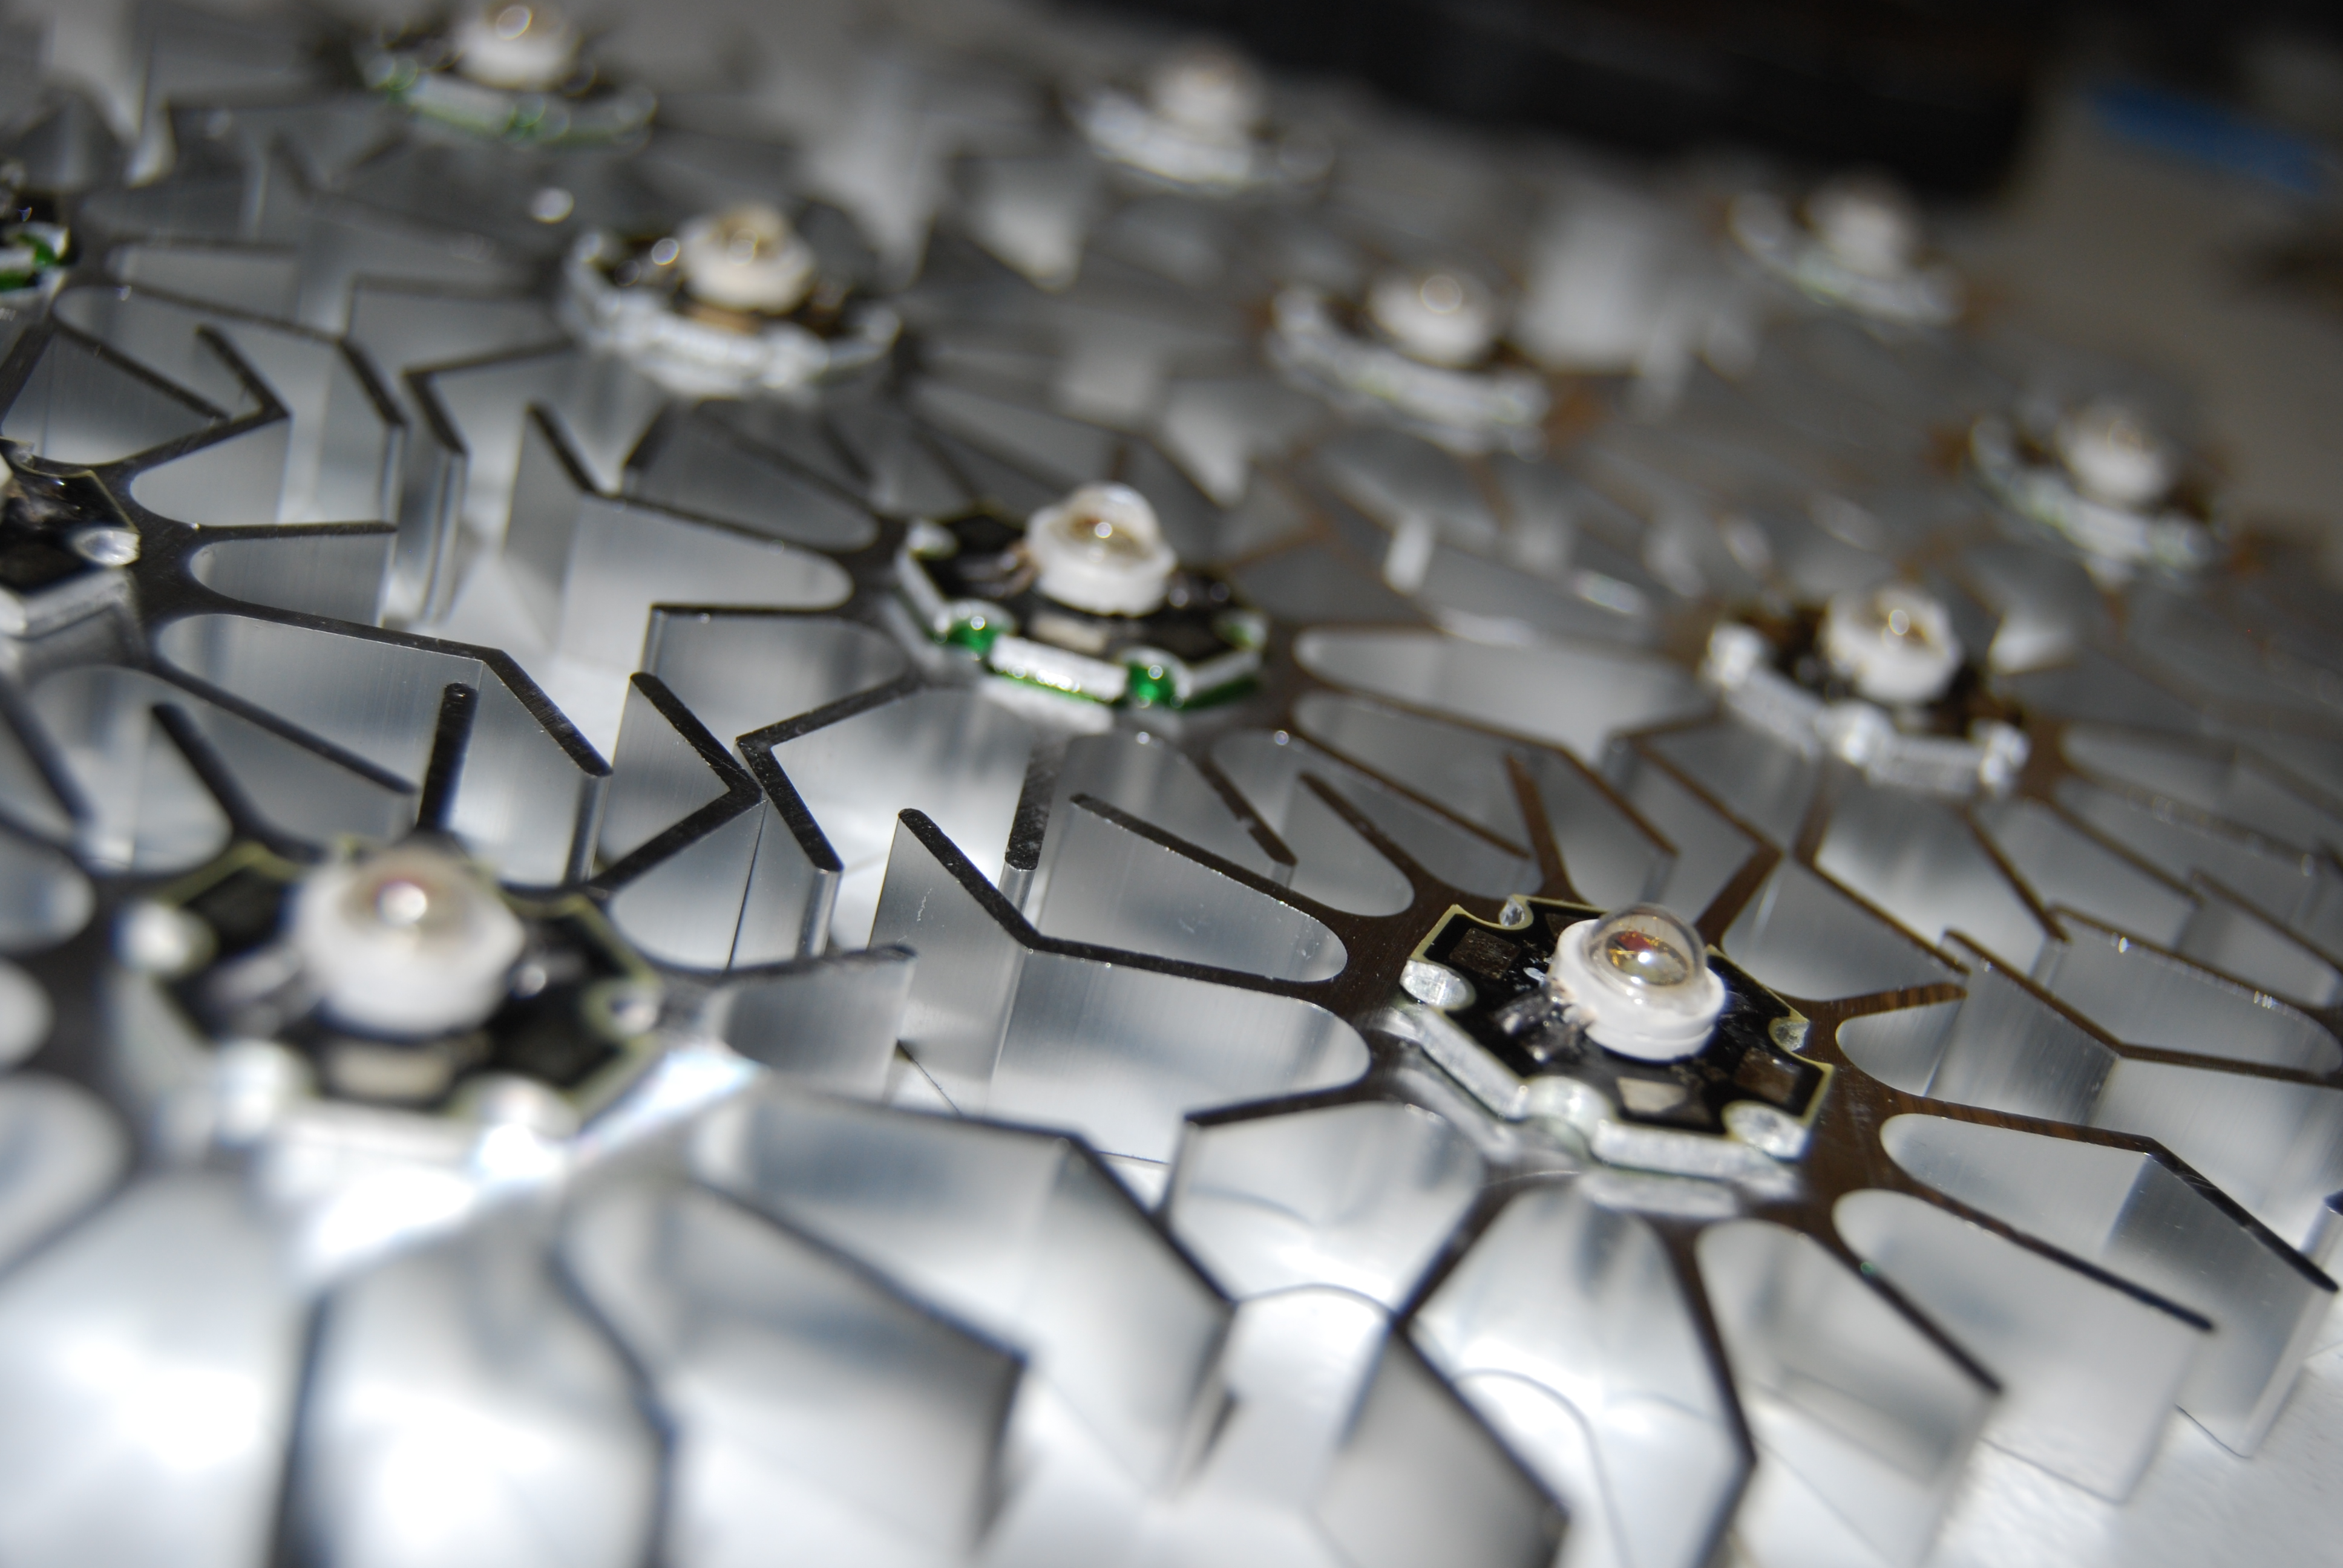
\includegraphics[width=5cm]{bilder/handarbeit3.JPG}
    \end{column}
  \end{columns}
  \begin{columns}
    \begin{column}{5cm}
      \begin{block}{Hardware}
        \begin{itemize}
        \item 100 lamps available
        \item > 100 plastic boxes for versatile inside/outside installations
        \end{itemize}
      \end{block}
    \end{column}
    \begin{column}{5cm}
    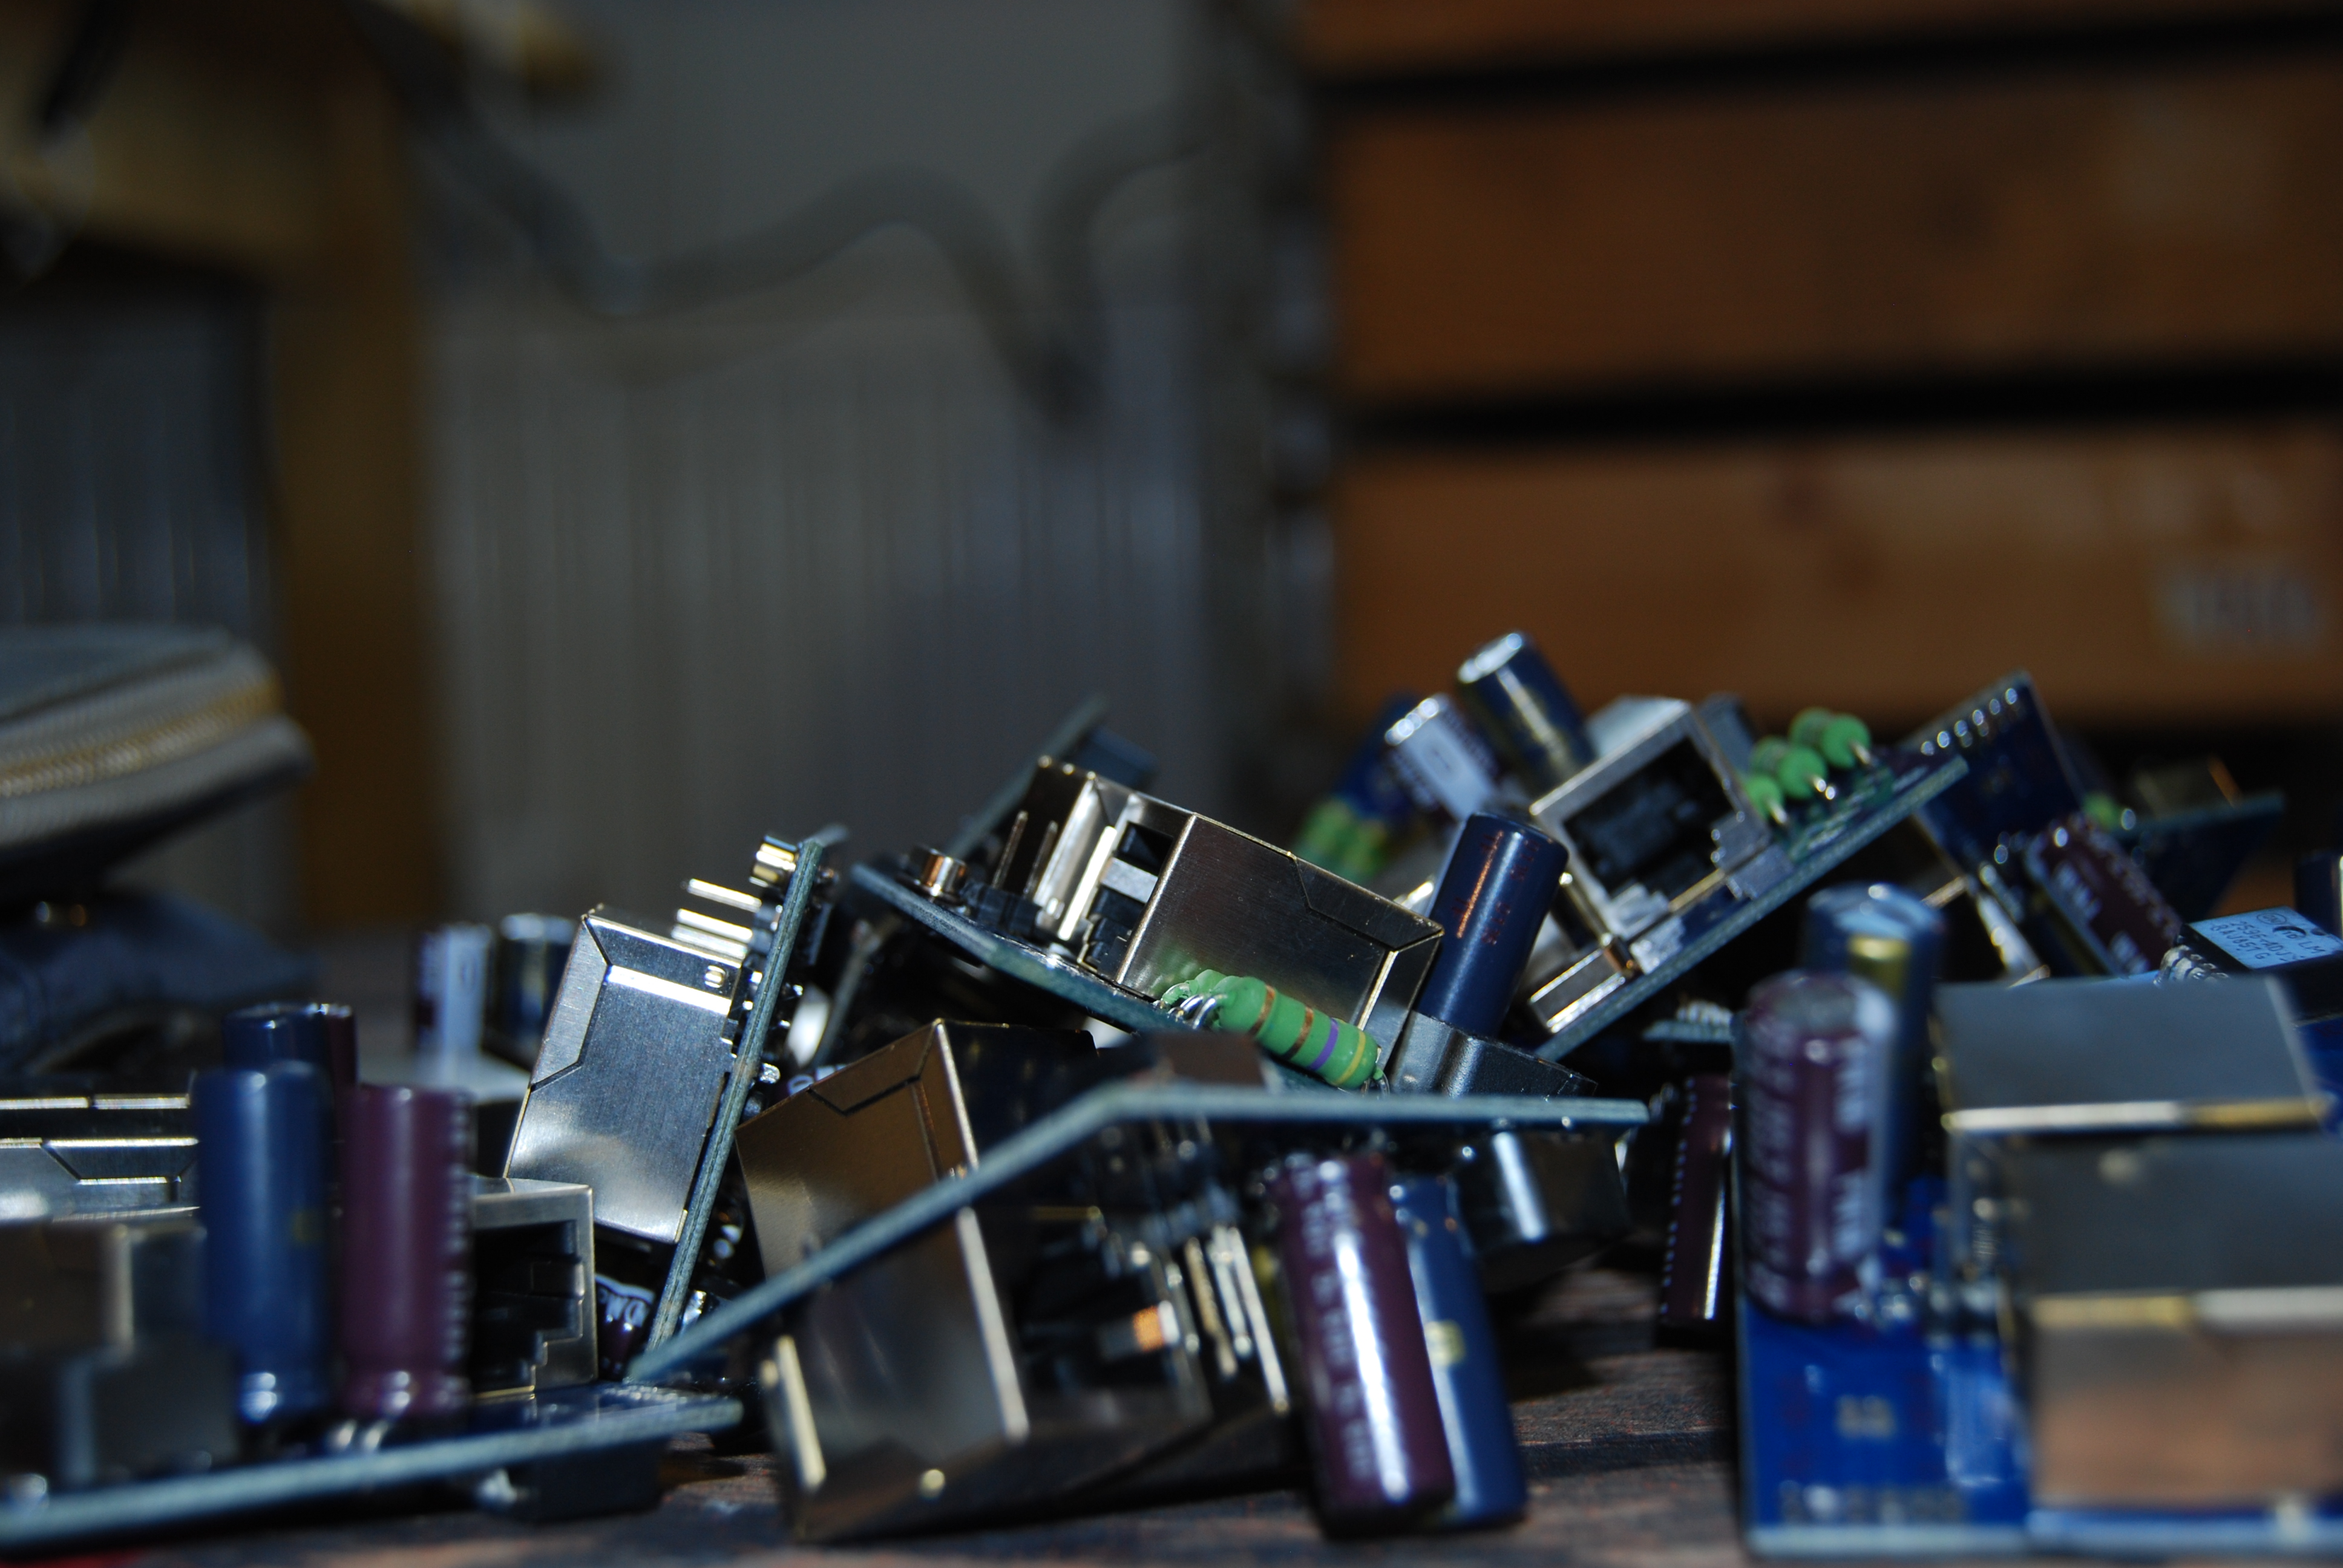
\includegraphics[width=5cm]{bilder/handarbeit2.JPG}
    \end{column}
  \end{columns}
\end{frame}
\begin{frame}{acab anywhere}
  \begin{columns}
    \begin{column}{5cm}
      \begin{block}{Finances}
        \begin{itemize}
        \item Start early\ldots
        \item Support from CCC
	\item Municipal sources
        \item Donations: Pixelpaten (lamp godfathers)
        \end{itemize}
      \end{block}
    \end{column}
    \begin{column}{5cm}
      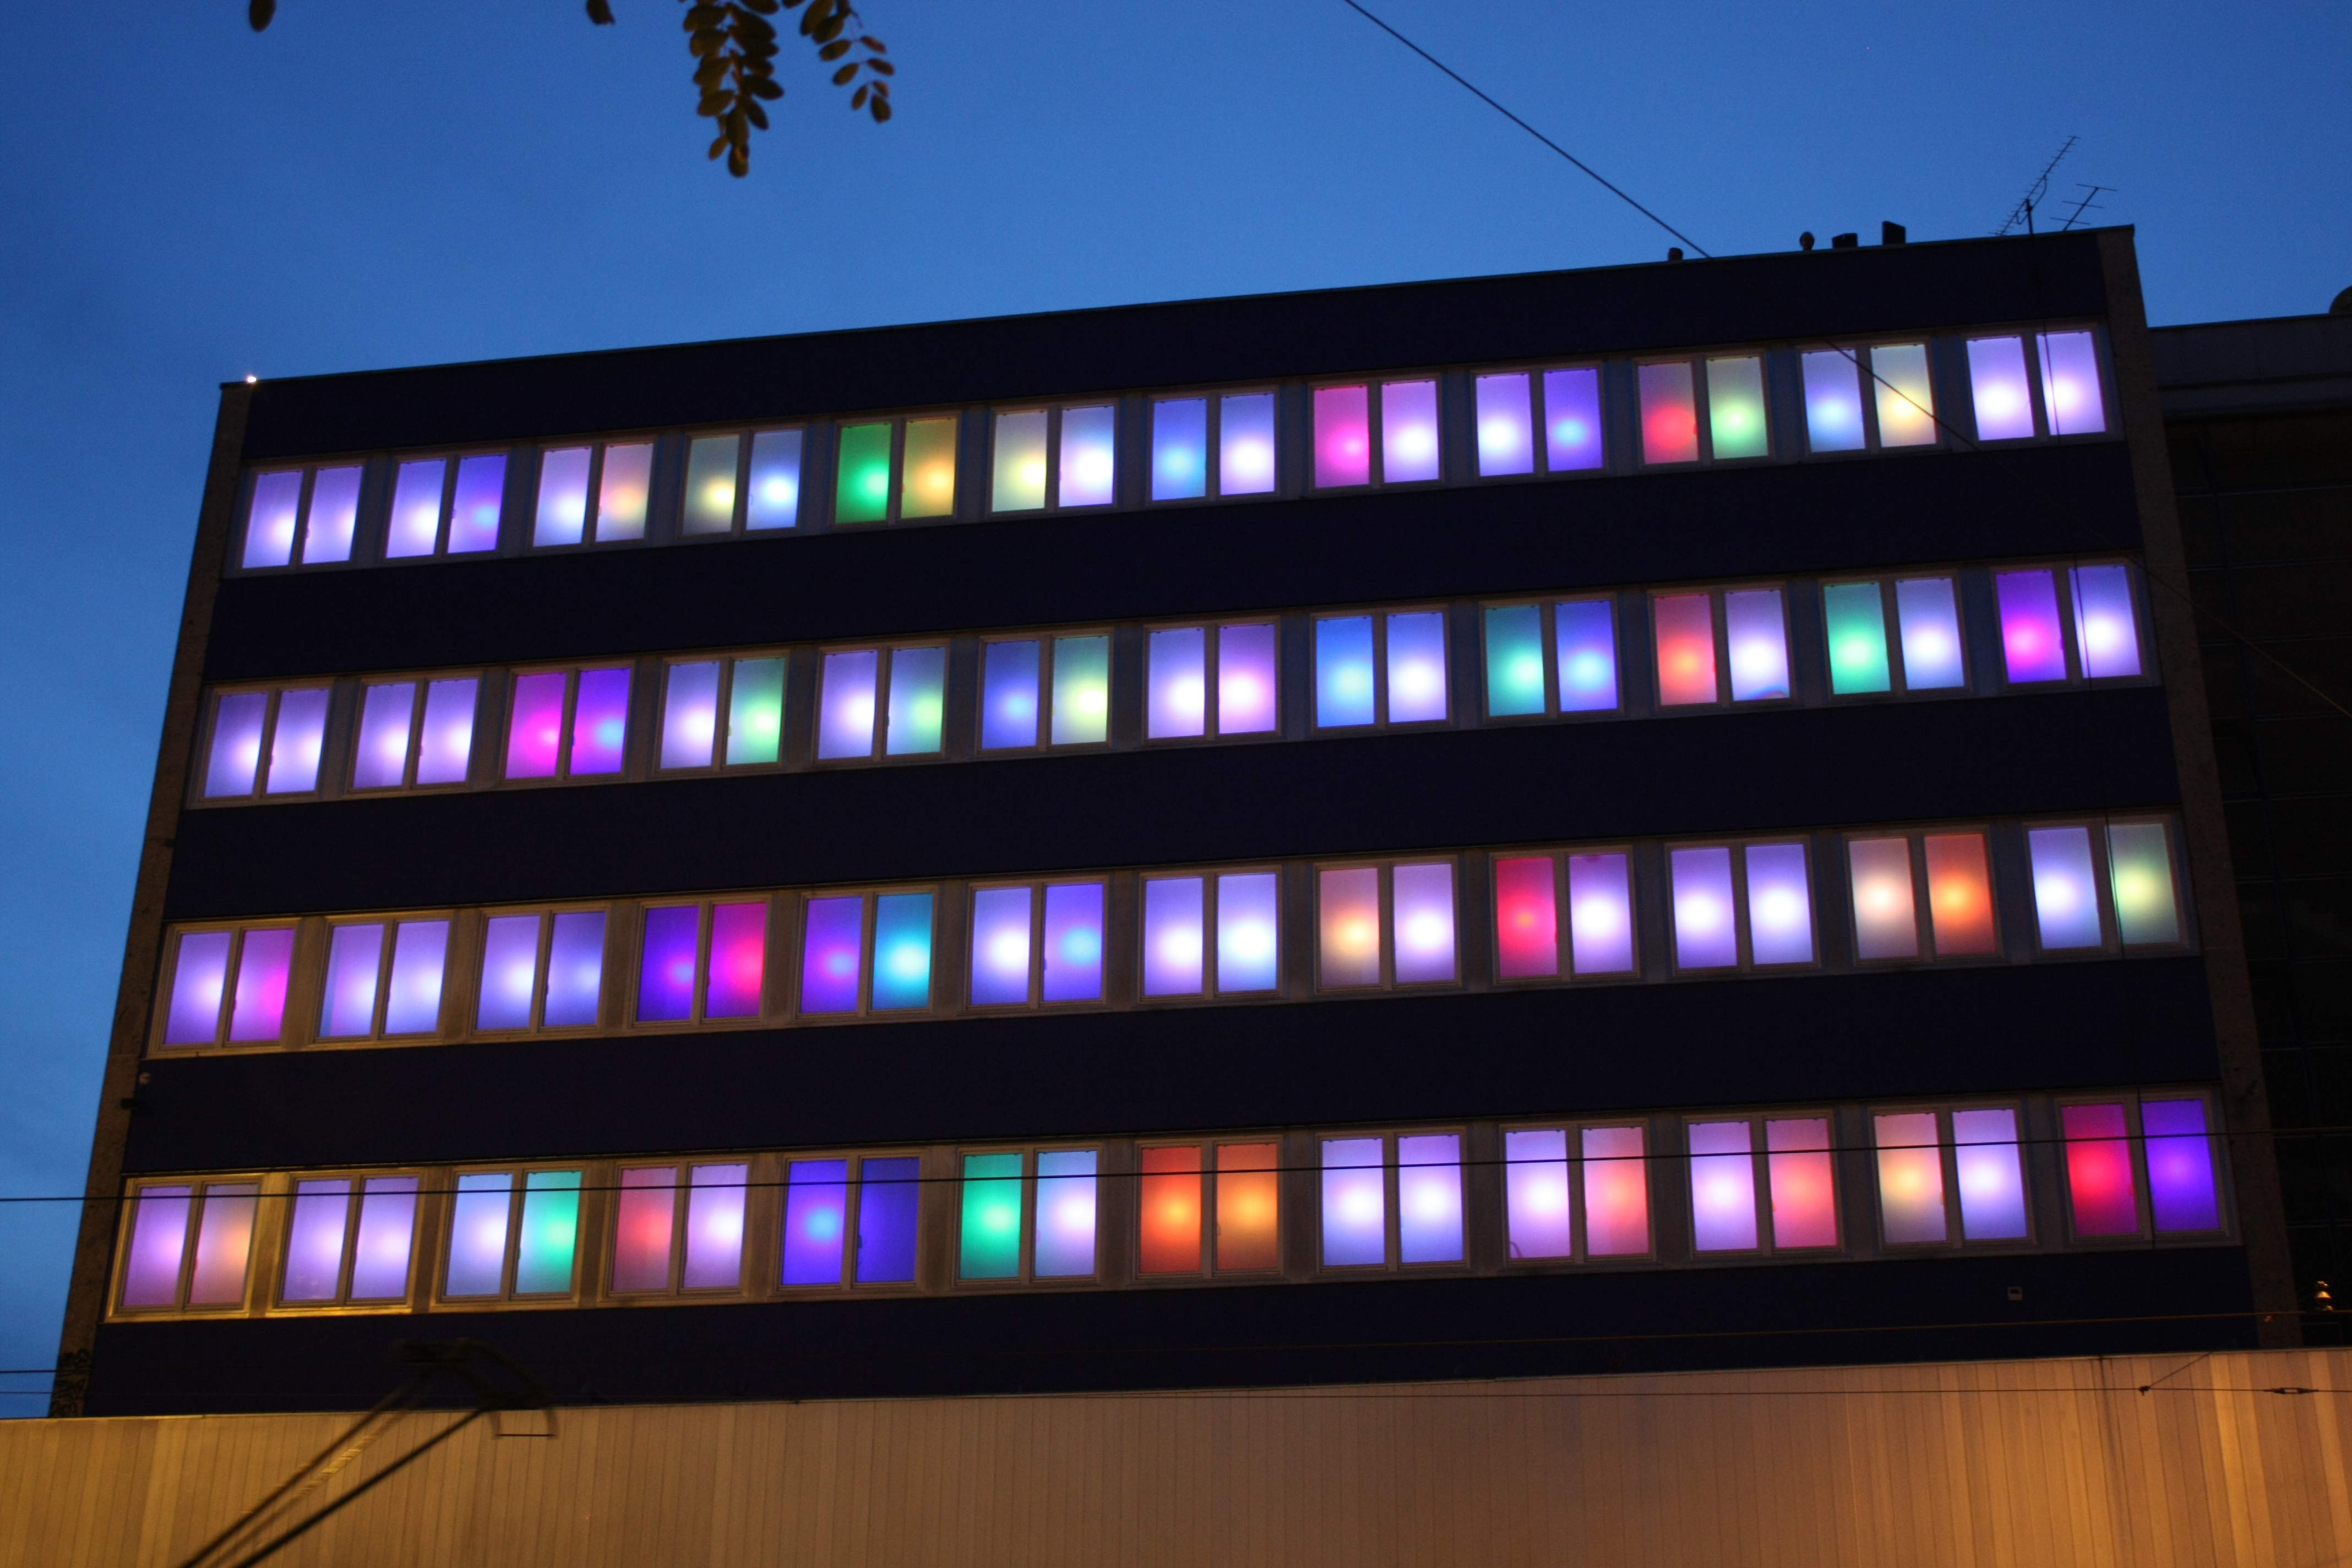
\includegraphics[width=5cm]{bilder/pixelpaten.JPG}
    \end{column}
  \end{columns}
%\hskip 0.7cm 
  \begin{columns}
    \begin{column}{5cm}
      \begin{block}{Time}
        \begin{itemize}
        \item Don't underestimate lead times for components 
        \item Leave enough time for some experiments
        \end{itemize}
      \end{block}
    \end{column}
    \begin{column}{5cm}
      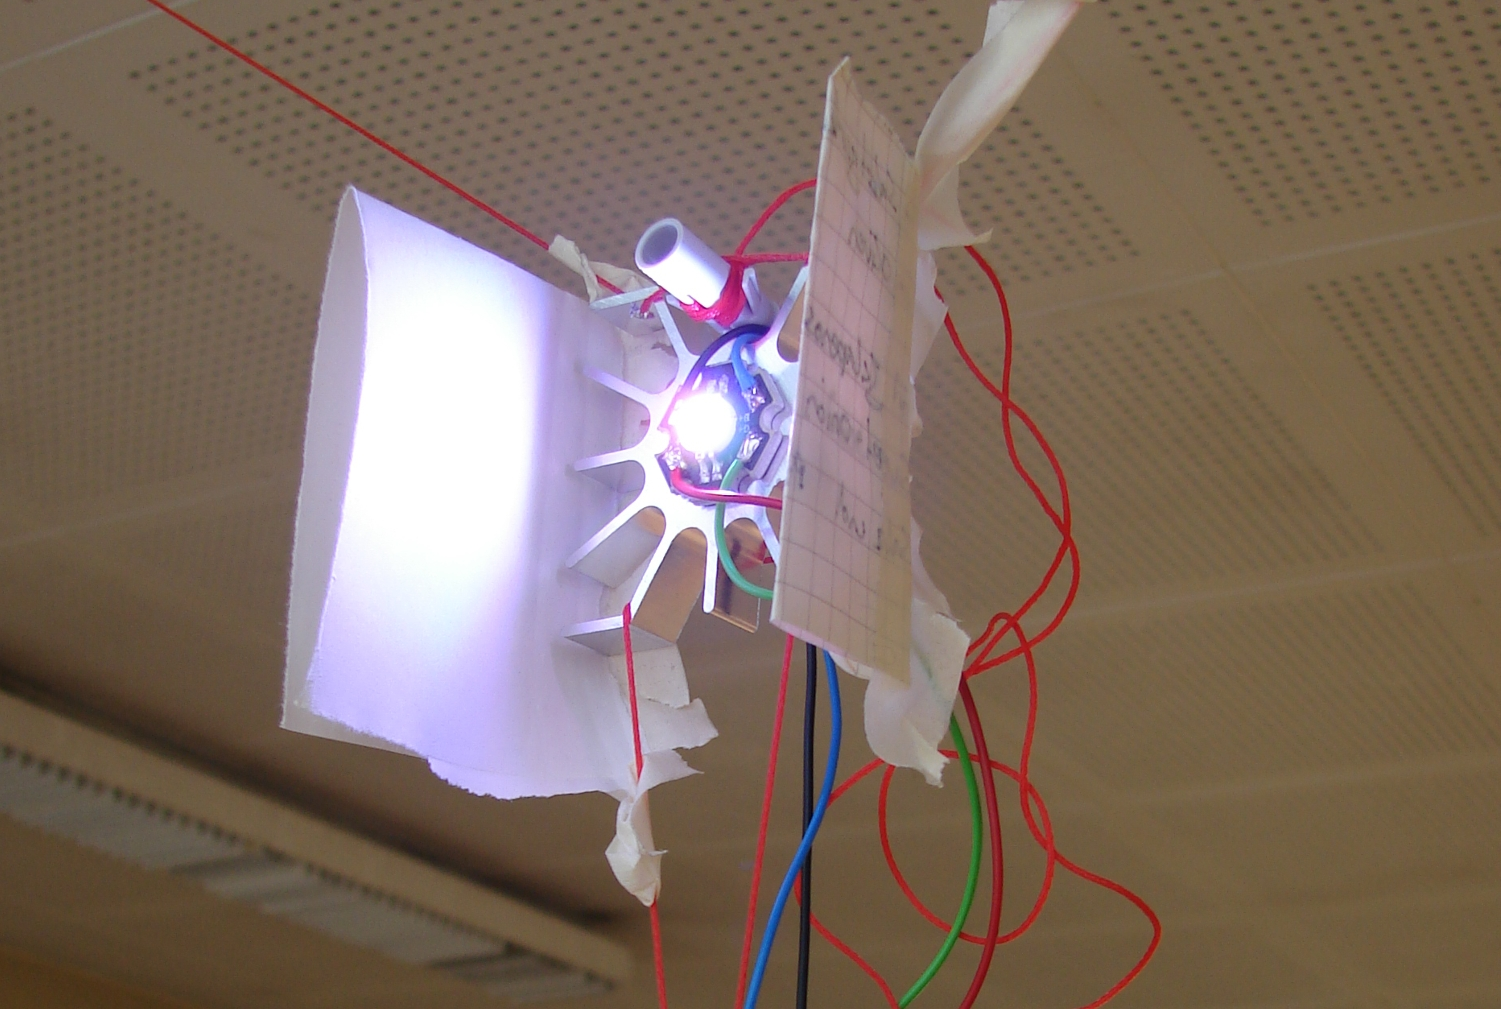
\includegraphics[width=5cm]{bilder/rumprobieren.JPG}
    \end{column}
  \end{columns}
\end{frame}

\section{Contact}
\begin{frame}{Contact Overview}
  \begin{block}{IRC}
    \begin{itemize}
	\item {\tt \#acab @ ray.blafasel.de}
    \end{itemize}
  \end{block}
  \begin{block}{Information}
    \begin{columns}
      \begin{column}{6.5cm}
        \begin{itemize}
        \item \url{http://acab.muc.ccc.de/}
        \item \url{http://muc.ccc.de/}
	\item \url{info@muc.ccc.de}
	\item \url{presse@muc.ccc.de}
        \end{itemize}
      \end{column}
      \begin{column}{4cm}
        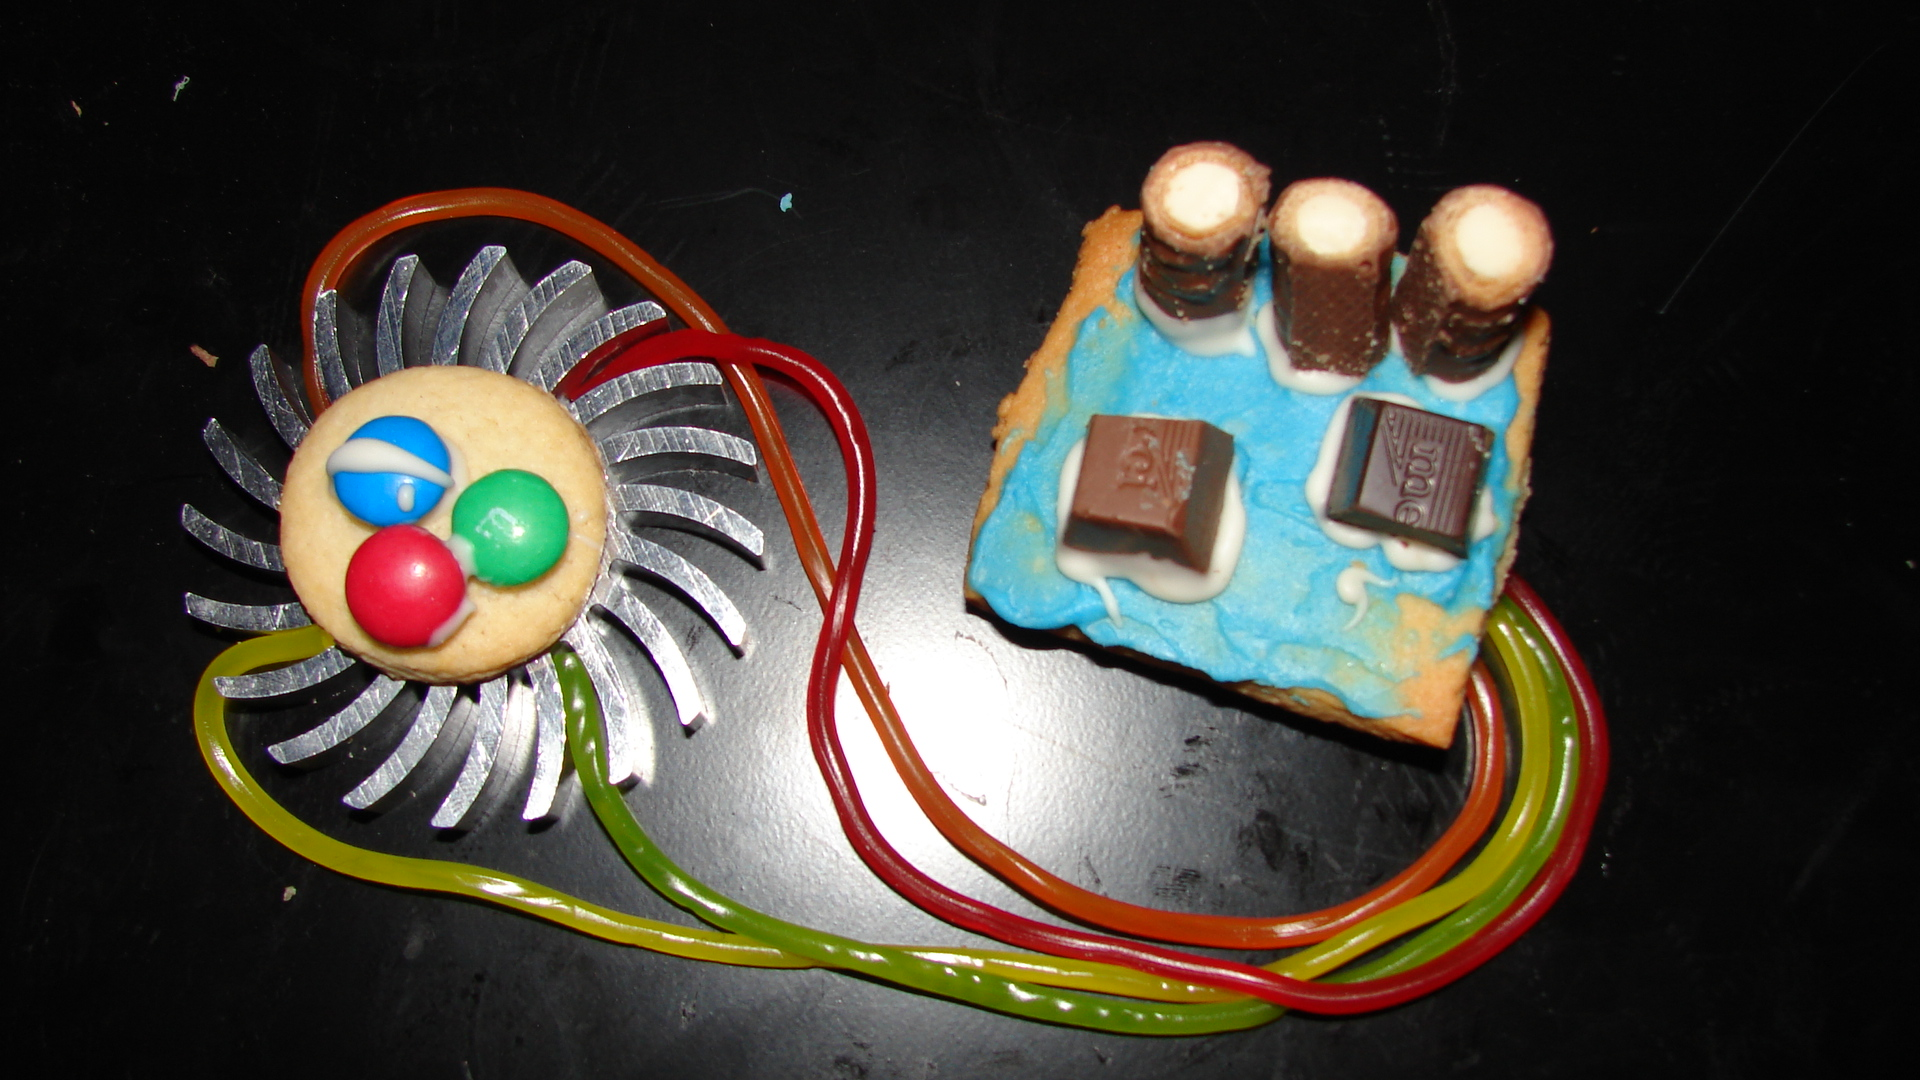
\includegraphics[width=3.4cm, clip, trim 2cm 0 2cm 0]{bilder/kekslampe.JPG}
      \end{column}
    \end{columns}
  \end{block}
  \begin{block}{Code}
    \begin{itemize}
      \item \url{https://github.com/muccc/}
    \end{itemize}
  \end{block}
\end{frame}
\end{document}
